\documentclass[10.5pt]{config}
% 本实验报告采用 署名-相同方式共享 4.0 国际许可协议 (CC BY-SA 4.0)
\usepackage{multirow}
\usepackage{wrapfig}
\usepackage{setspace}
\usepackage{titlesec}
\usepackage{ctex}
\usepackage{graphicx} % 用于插入图片
\usepackage{float}    % 用于控制图片位置
\usepackage{makecell}
\usepackage{tikz}
\usepackage{enumitem} % 用于更灵活的列表环境
\usetikzlibrary{arrows.meta}

\titleformat{\subsubsection}[block]  % 设置为块级标题（自动换行）
{\normalfont\bfseries}{\thesubsubsection}{1em}{} 
\titlespacing*{\subsubsection}{1.5em}{3.25ex}{1.5ex}  % 调整缩进：左缩进2em
\setstretch{1.5}

% --- 请在这里填写您的个人信息 ---
\major{} % 专业
\name{}
\partner{} % 签名栏
\stuid{}
\date{} % 可根据实际实验日期修改
\lab{}
\grades{}
\course{电工电子学实验}
\instructor{} % 指导老师
\exptype{基础实验} % 实验类型
\expname{集成运算放大器应用(二)} % 按照PPT要求修改实验名称


\begin{document}

\makeheader % 首页头部

\section{实验目的}

\begin{enumerate}[label=\arabic*., leftmargin=2em]
    \item 掌握幅值比较器的电路组成及工作原理。
    \item 掌握用集成运放构成的方波、三角波发生器的工作原理和性能。
    \item 了解压控脉宽调制电路的组成和工作原理。
\end{enumerate}

\section{实验设备}
\begin{enumerate}[label=\arabic*., leftmargin=2em]
    \item 模拟电子技术实验箱
    \item 双踪数字示波器
    \item 函数信号发生器
    \item 直流电源
    \item 数字式万用表
\end{enumerate}

\section{实验原理}

\subsection*{1. 同相输入电压比较器}
如图所示为集成运放构成的幅值比较器。运放工作在开环状态，输出为正、负饱和电平。反相端接参考电压 $U_R$，输入信号 $u_i$ 从同相端输入。当 $u_i > U_R$ 时，$u_o = U_{OH}$；当 $u_i < U_R$ 时，$u_o = U_{OL}$。当输入为一定幅度的正弦波时，比较器将输入正弦波变换为矩形波输出。

\begin{figure}[H] 
    \centering 
    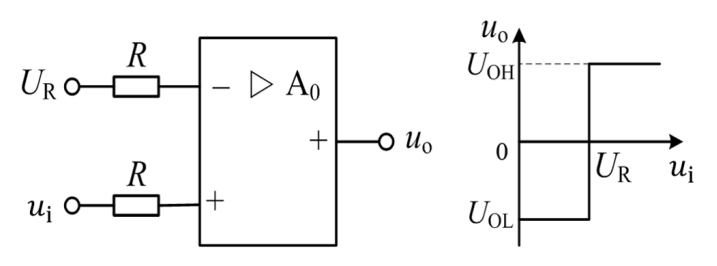
\includegraphics[width=0.7\textwidth]{figures/bijiaoqi.png} 
    \caption{同相输入幅值比较器和电压传输特性曲线}
    \label{fig:bijiaoqi}
\end{figure}

\subsection*{2. 由集成运放构成的方波、三角波发生电路和压控脉宽调制电路}
前两级中，$A_1$ 为同相输入过零滞回比较器，$u_{o2}$ 为其输入信号；$A_2$ 构成积分器，$u_{o1}$ 为其输入。比较器、积分器连接成闭合环路，输出方波和三角波。理论周期和频率计算公式如下：
\begin{equation*}
    T = 4R_f C_f \frac{R_1}{R_2}
\end{equation*}
\begin{equation*}
    f = \frac{1}{T} = \frac{R_2}{R_1} \frac{1}{4 R_f C_f}
\end{equation*}

电路中 $A_3$ 构成压控脉宽调制电路。它是一个电压比较器，通过改变参考电压 $U_R$ 大小将输入的三角波变换成输出脉宽可变（即占空比可变）的矩形波。

\begin{figure}[H] 
    \centering 
    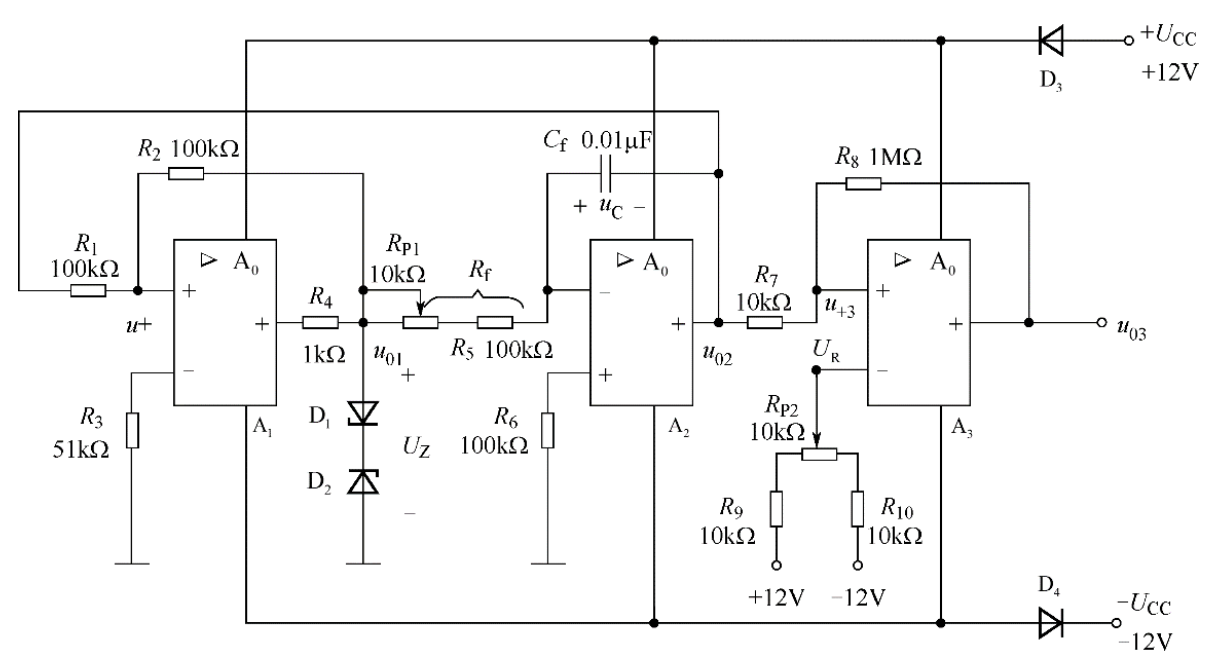
\includegraphics[width=0.8\textwidth]{figures/fashengqi.png} 
    \caption{方波、三角波发生电路及压控脉宽调制电路原理图}
    \label{fig:fashengqi}
\end{figure}



\section{实验内容}

\begin{enumerate}[label=\arabic*., leftmargin=2em]
    \item \textbf{按图电路接线（同相输入电压比较器）：} 
    \begin{itemize}
        \item (1) $U_R$ 接直流电压 1V。输入 $u_i$ 分别加直流电压 0.5V 和 1.5V，用万用表测量相对应的输出电压 $u_o$，并记录 $u_i, u_o$ 值。
        \item (2) 观测波形变换。$U_R$ 不变，输入 $u_i$ 加入正弦信号 ($U_p = 5\text{V}, f = 100\text{Hz}$)，用示波器双踪同时显示 $u_i, u_o$ 波形，记录波形和参数（幅值，周期，特别标注 $u_o$ 高低电平转换时 $u_i$ 的大小位置）。
        \item (3) 观测传输特性曲线。对 (2) 的输入条件不变，将示波器设置成 XY 方式，显示电压传输特性曲线，记录曲线和输入转折门限电压，输出高、低电平值。
    \end{itemize}
    
    \item \textbf{按图电路接线（由集成运放构成的方波、三角波发生电路）：} 
    \begin{itemize}
        \item (1) 先连接 $A_1$、$A_2$ 两级电路，$A_3$ 级电路暂时不连。调节电位器 $R_{P1}$ 滑动头，使得 $R_{P1} = 0$，用示波器同时观察 $u_{o1}$ 和 $u_{o2}$ 波形，记录两波形，测量记录 $u_{o1}$ 和 $u_{o2}$ 的频率和幅值。
        \item (2) 保持 $R_{P1} = 0$, $R_2 = 100\text{k}\Omega$ 不变，将 $R_1$ 改为 $51\text{k}\Omega$，重复 (1) 的实验内容。
        \item (3) 保持 $R_1 = R_2 = 100\text{k}\Omega$，调节电位器 $R_{P1}$，观察并记录 $u_{o1}$ 和 $u_{o2}$ 的频率和幅值变化情况。
    \end{itemize}
    
    \item \textbf{按图电路接线，调试测量脉宽调制电路：} \\
    保持 $R_1 = R_2 = 100\text{k}\Omega$, $R_{P1} = 0$。连接好 $A_3$ 级电路。把 $u_{o2}$ 作为脉宽调制电路的输入电压，根据表 5.17-1（P172）改变参考电压 $U_R$ 值完成各项内容的测试。
\end{enumerate}


\section{实验数据记录与波形}

\subsection*{1. 同相输入电压比较器测试记录}

实验1（1）：

\textbf{静态电压测试 ( $U_R = 1\text{V}$ )：}
\begin{itemize}
    \item 当 $u_i = 0.5\text{V}$ 时，实测输出电压 $u_o =-12.1132$ V
    \item 当 $u_i = 1.5\text{V}$ 时，实测输出电压 $u_o =+10.7428 $ V
\end{itemize}

实验1（2）：

\begin{figure}[H] 
    \centering 
    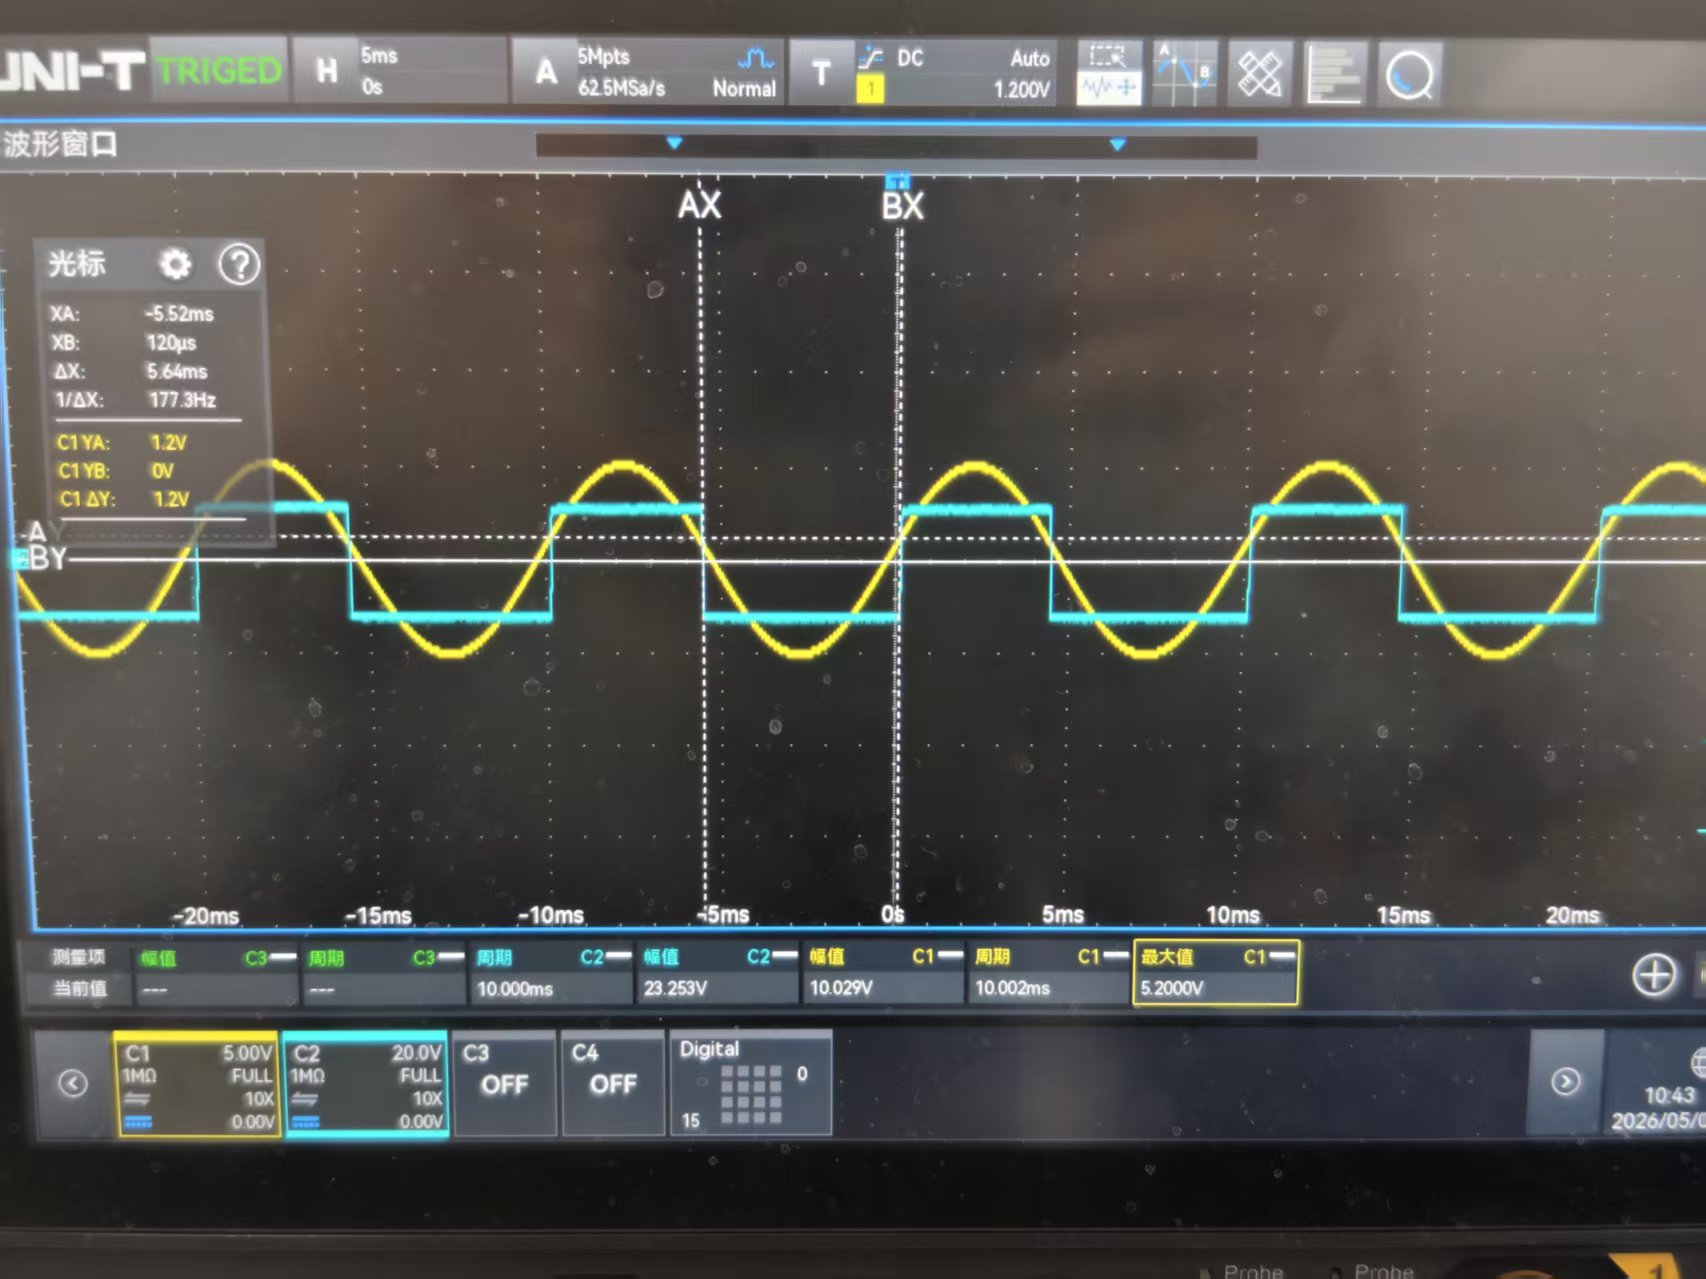
\includegraphics[width=0.45\textwidth]{figures/bijiaoqi_yt.jpg} 
    \caption{电压比较器输入与输出波形 (y-t 模式)}
\end{figure}

从图中读出正弦波幅值为10.029V，方波幅值为23.253V；周期为10.002ms，两次高低电平转换时间间隔为5.64ms，4.362ms。

实验1（3）：

\begin{figure}[H] 
    \centering 
    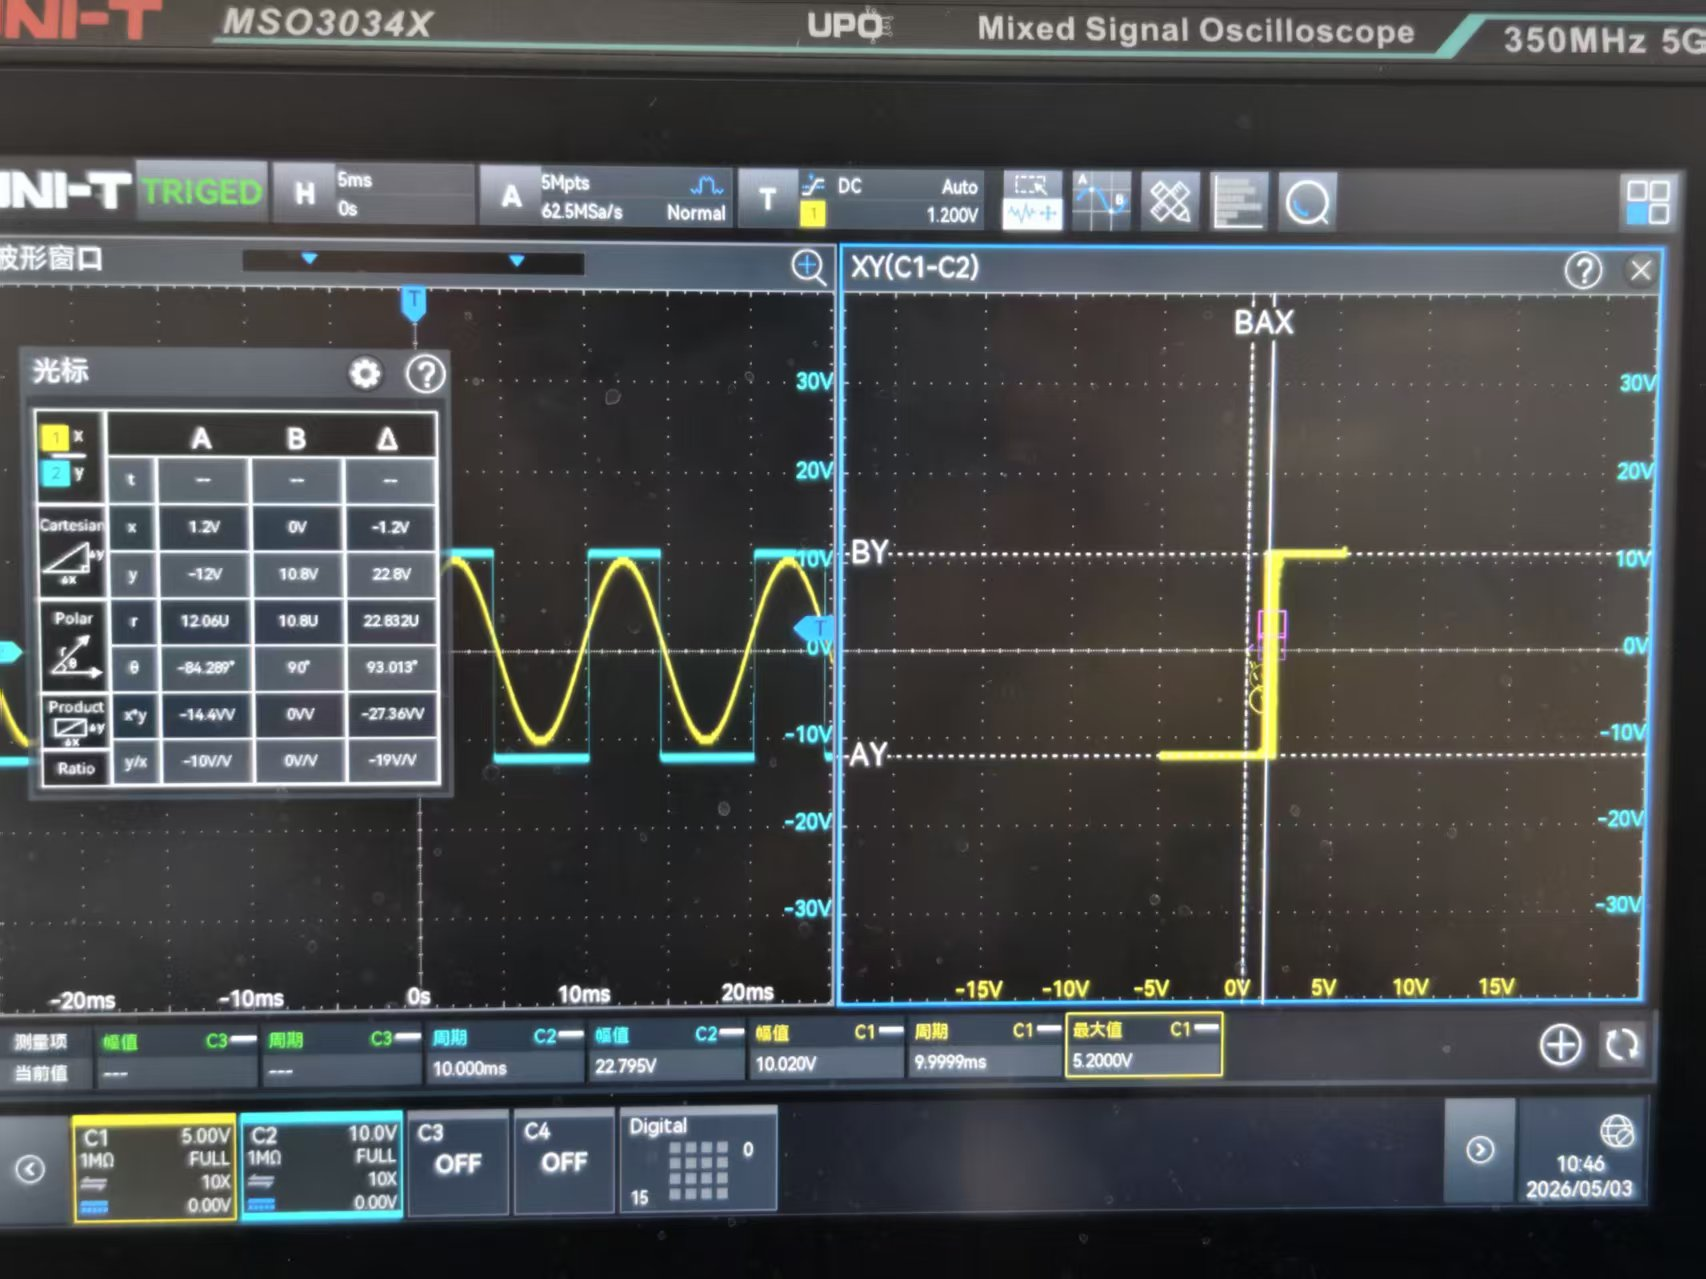
\includegraphics[width=0.45\textwidth]{figures/bijiaoqi_xy.jpg} 
    \caption{电压比较器传输特性曲线 (x-y 模式)}
\end{figure}

输出转折门限电压为1.2V，输出高电平值为10.8V，输出低电平值为-12V。

\subsection*{2. 方波、三角波发生电路测试记录}

实验2（1）：

\begin{figure}[H] 
    \centering 
    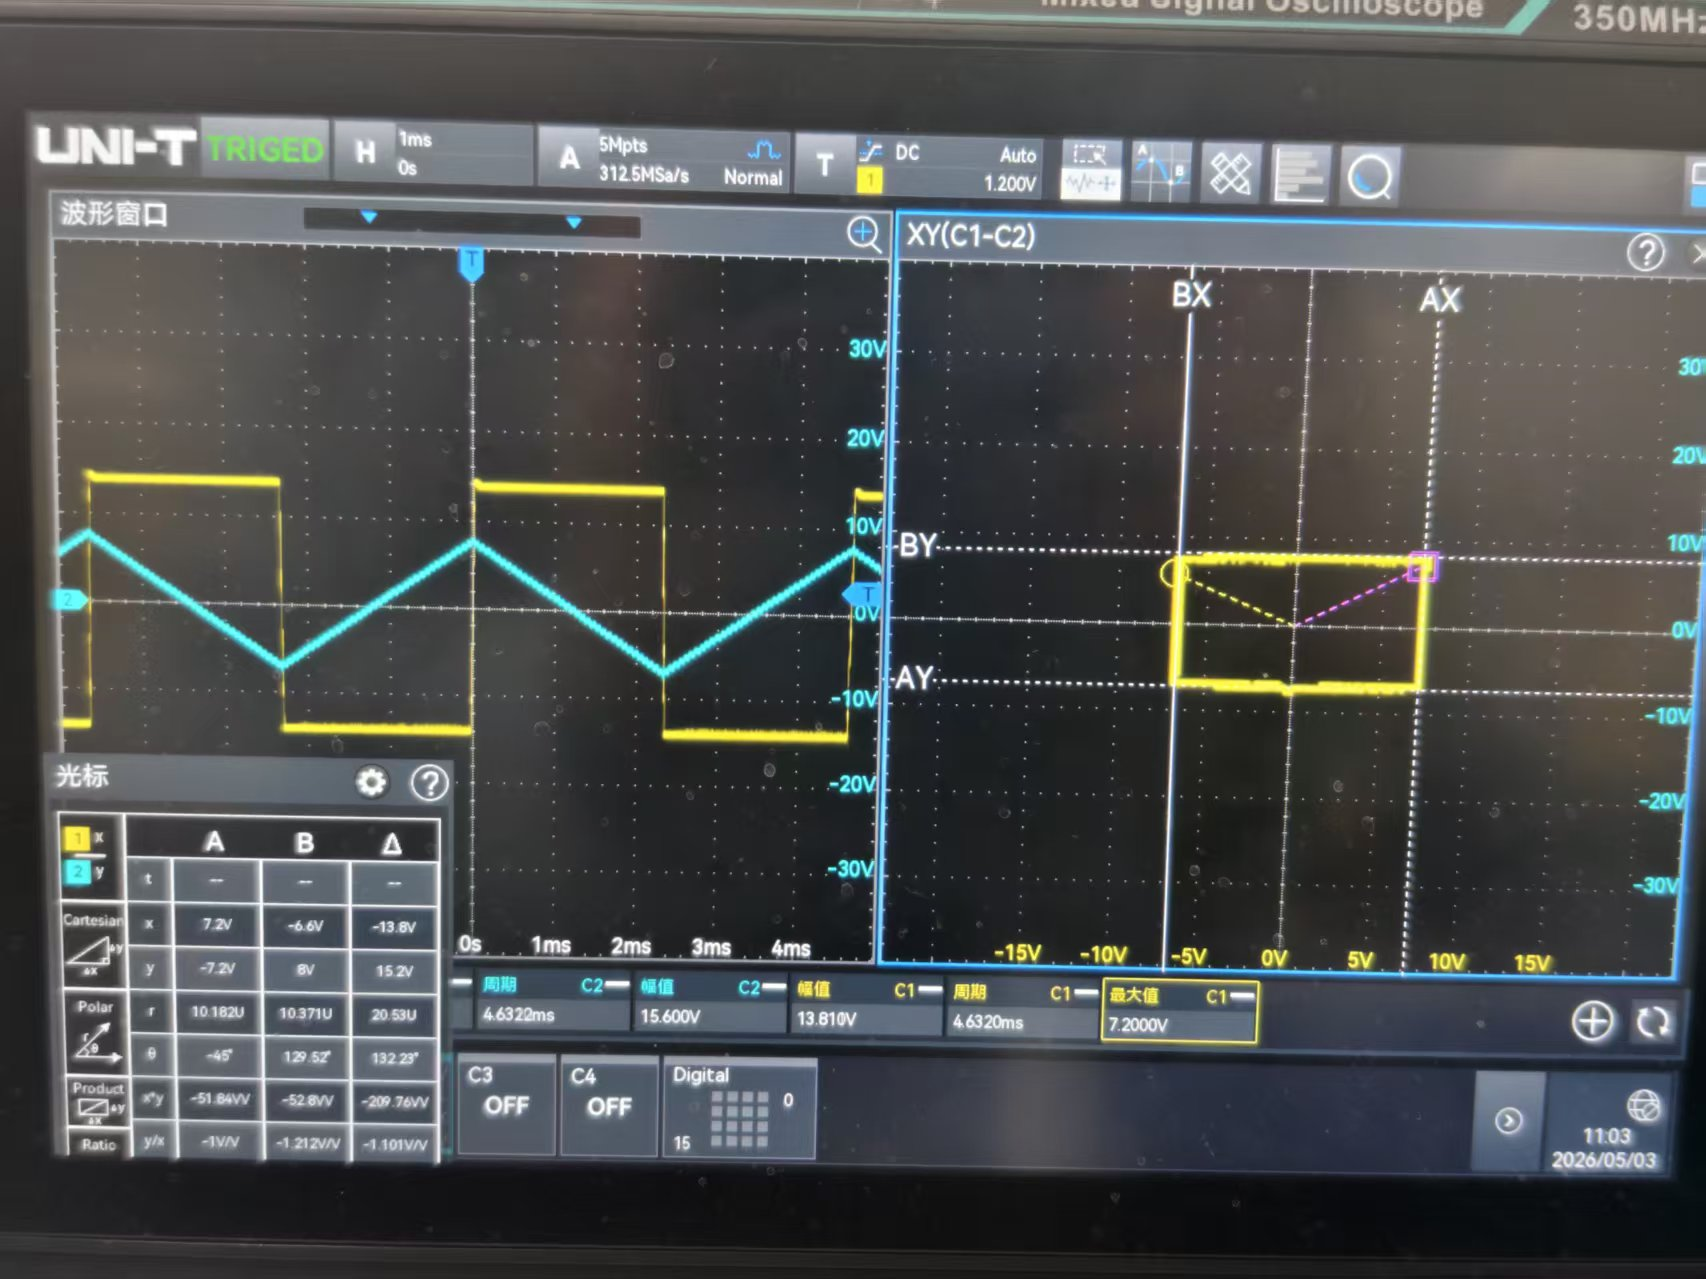
\includegraphics[width=0.45\textwidth]{figures/rp0.jpg} 
    \caption{方波与三角波波形图 ($u_{o1}$ 与 $u_{o2}$)}
\end{figure}

$Rp1=0$时，从图中得到方波幅值为13.810V，三角波幅值为15.600V，周期为4.6320ms。

实验2（2）：

将$R_1$改为51$k\Omega$

\begin{figure}[H] 
    \centering 
    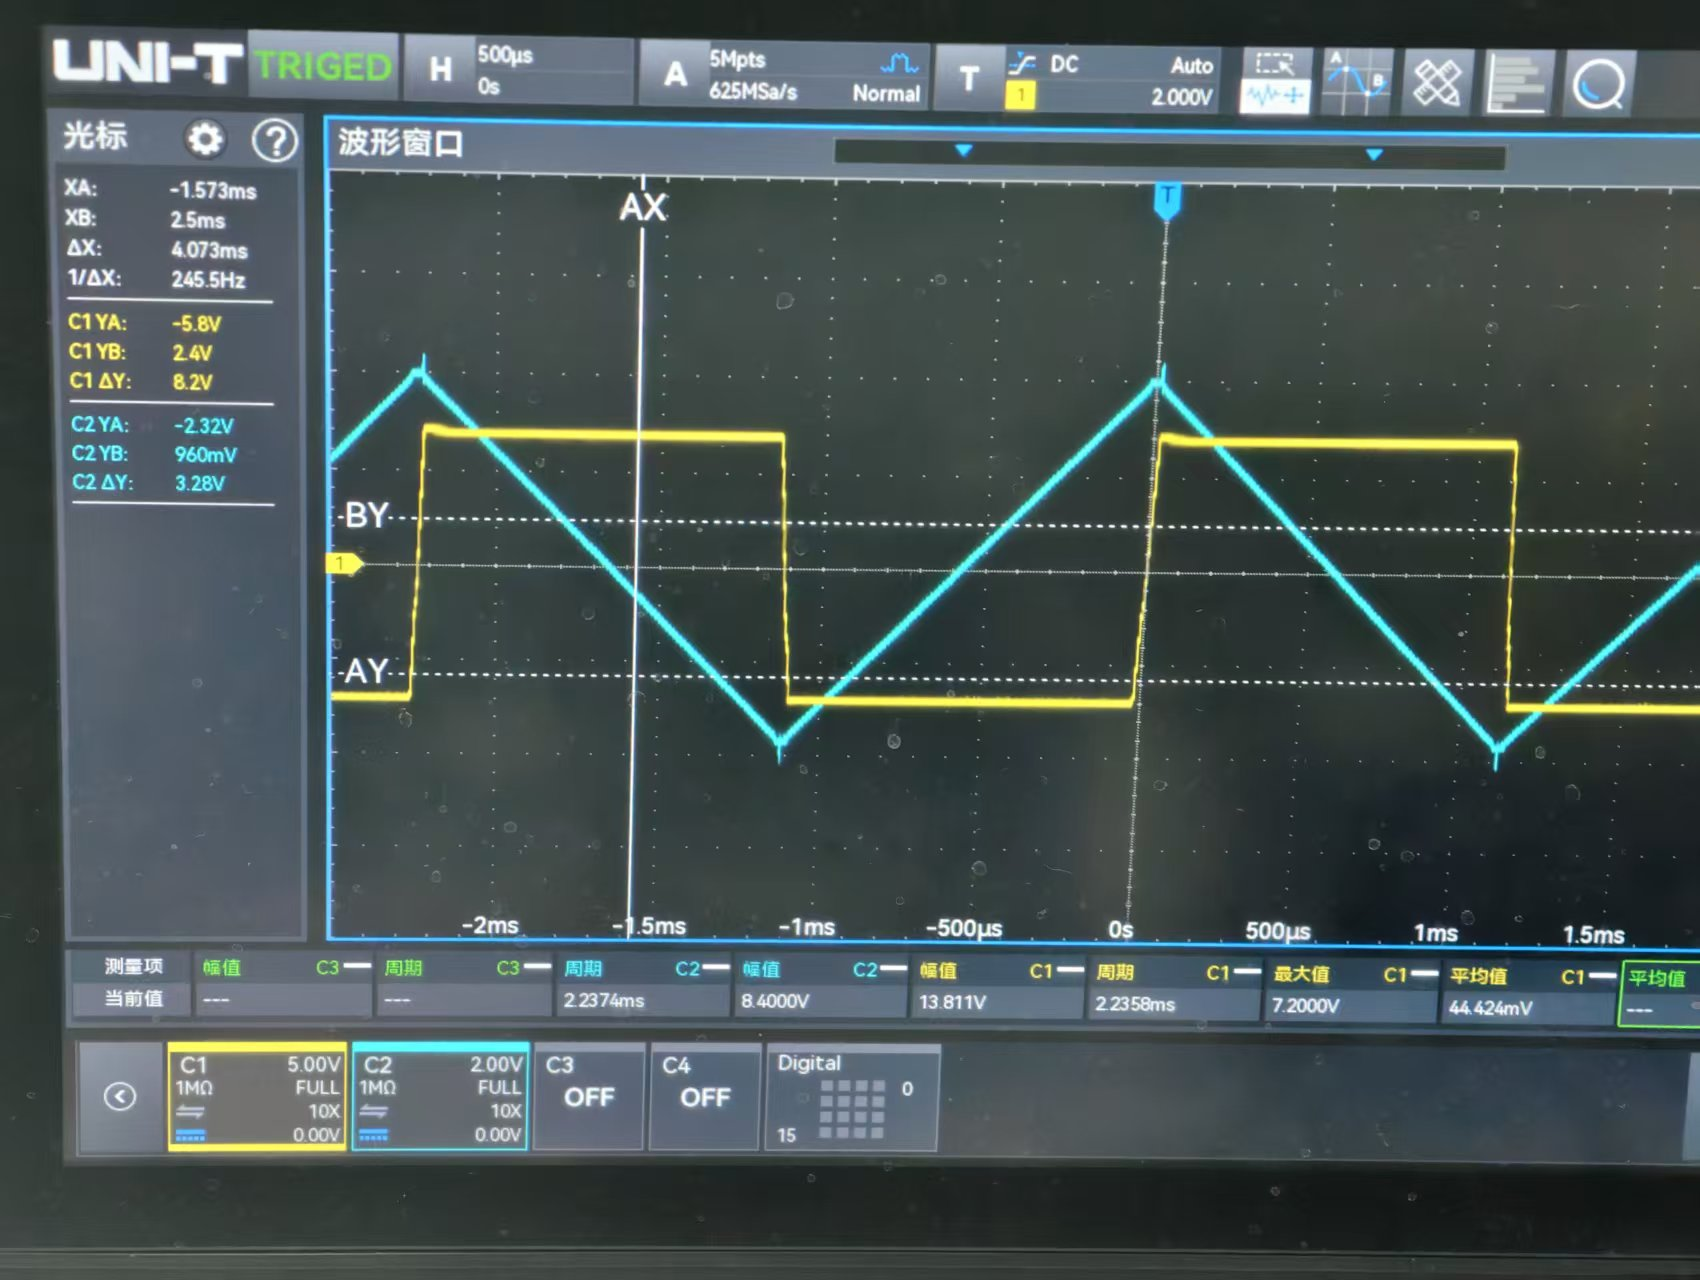
\includegraphics[width=0.45\textwidth]{figures/51k.jpg} 

\end{figure}

$Rp1$逐渐调大

\begin{figure}[H] 
    \centering 
    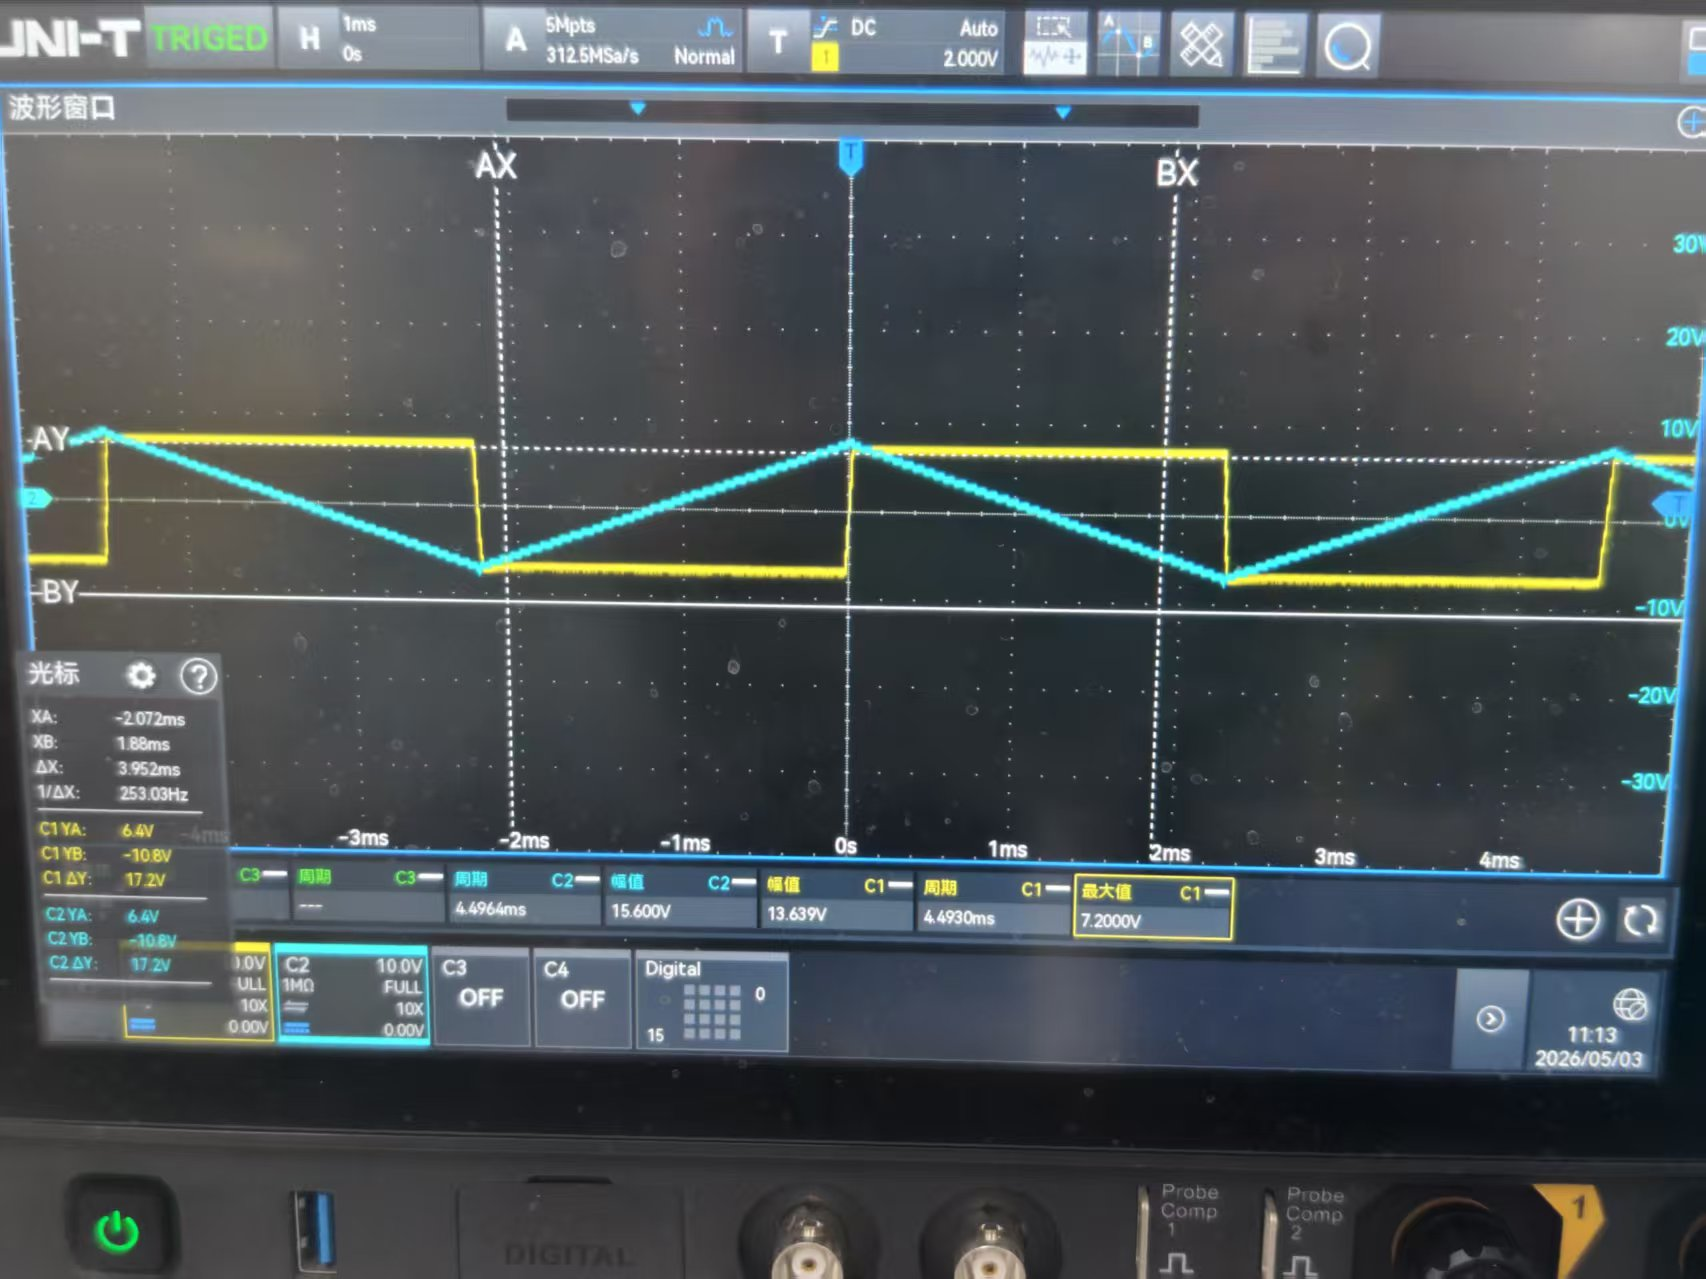
\includegraphics[width=0.45\textwidth]{figures/rp1.jpg} 

\end{figure}

方波幅值为13.810V，三角波幅值为15.600V，周期为4.4930ms。

\begin{figure}[H] 
    \centering 
    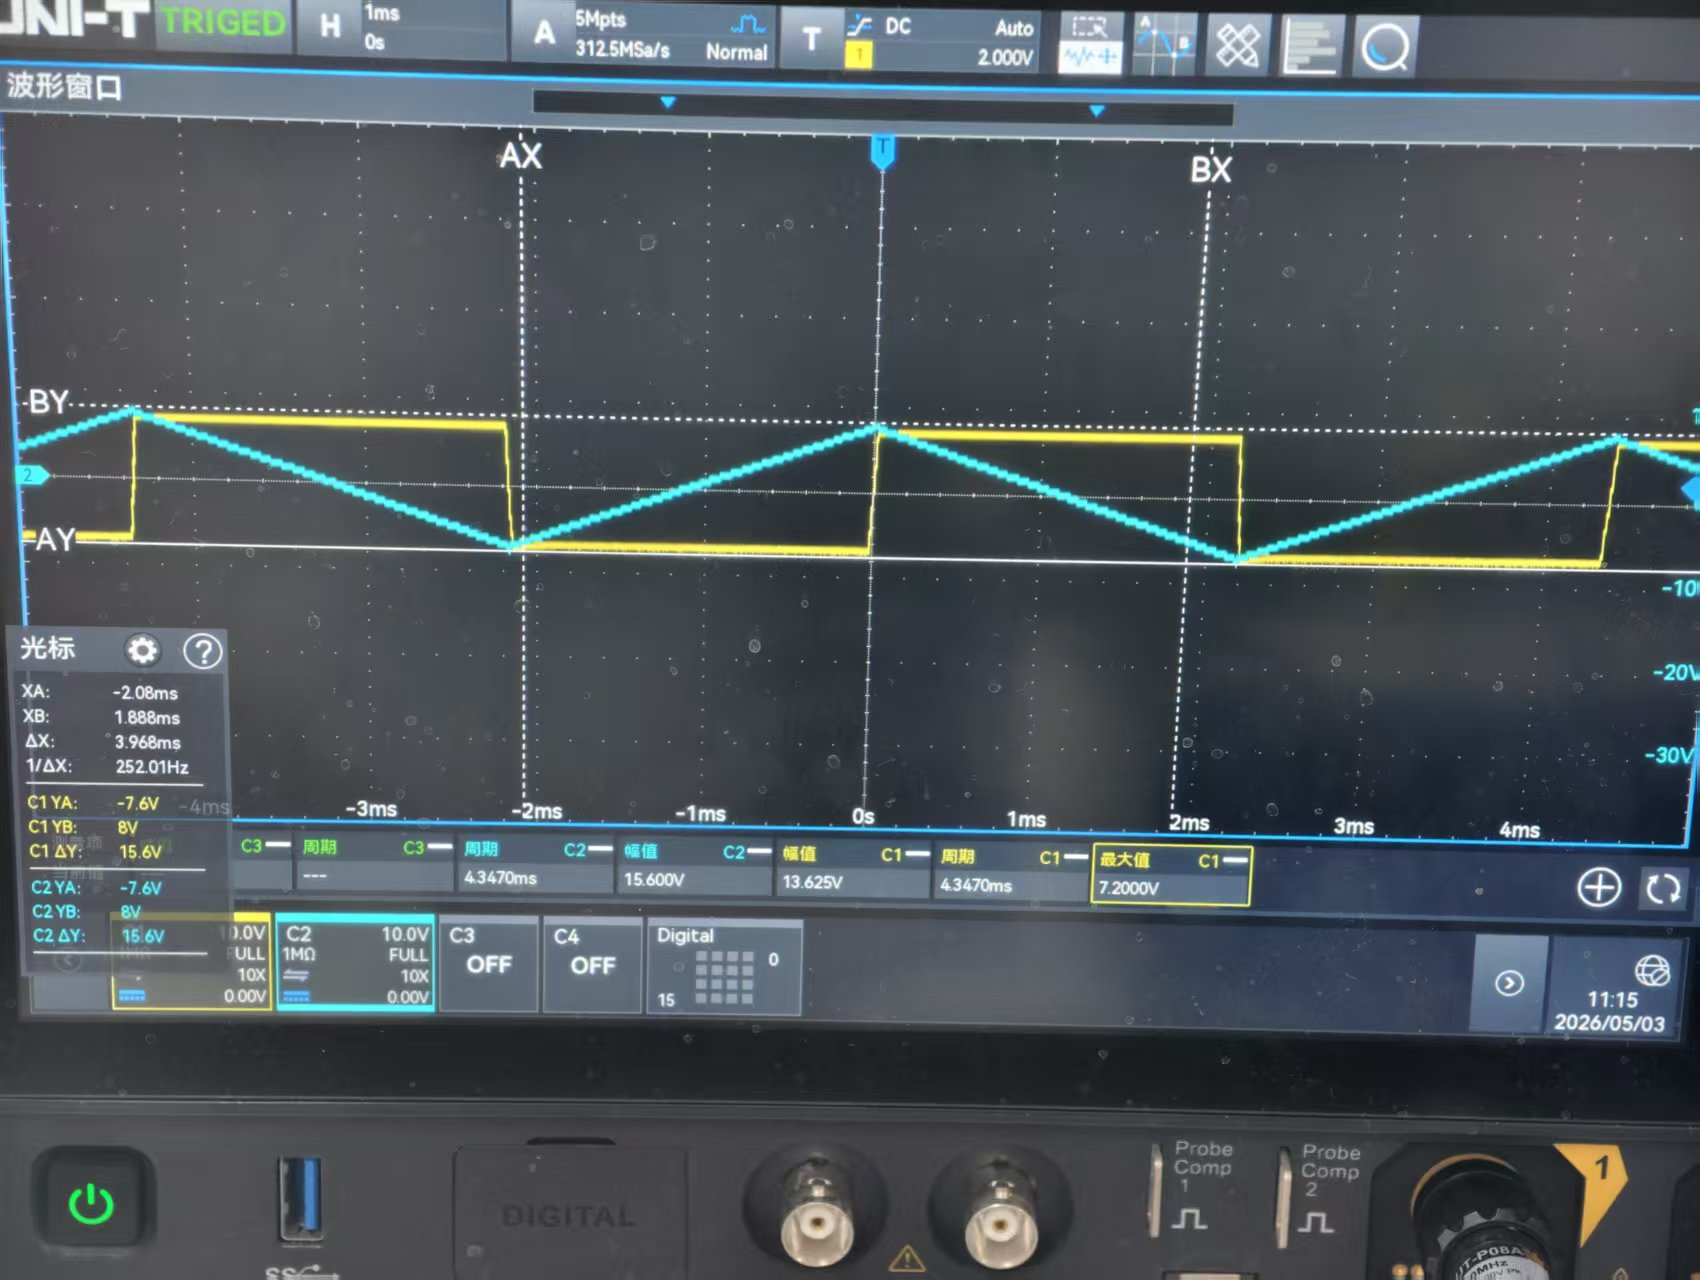
\includegraphics[width=0.45\textwidth]{figures/rp2.jpg} 

\end{figure}

方波幅值为13.810V，三角波幅值为15.600V，周期为4.3470ms。

\begin{figure}[H] 
    \centering 
    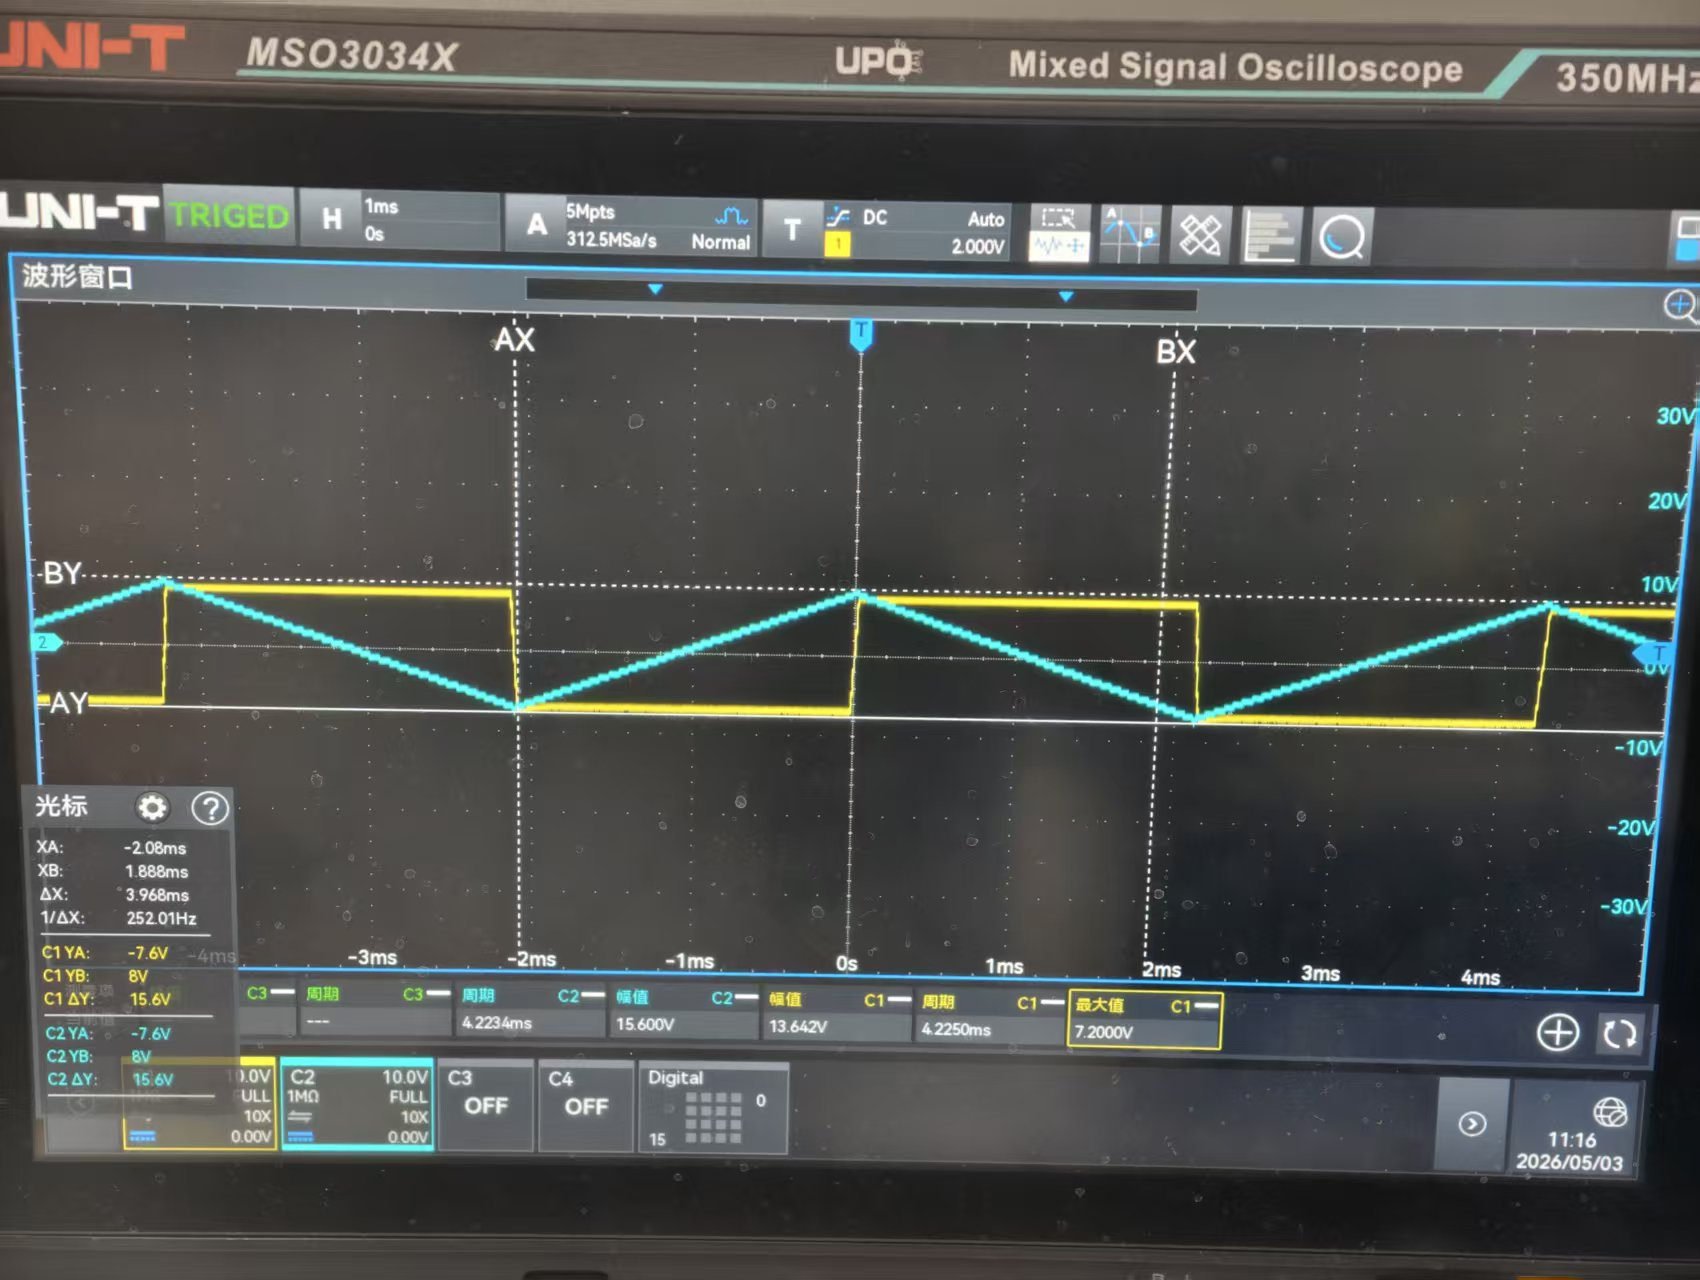
\includegraphics[width=0.45\textwidth]{figures/rp3.jpg} 

\end{figure}

方波幅值为13.810V，三角波幅值为15.600V，周期为4.2250ms。

可以看出，当$Rp1$逐渐调大，信号的幅值基本不变，但周期不断减小。



\subsection*{3. 压控脉宽调制电路测试记录}

\begin{table}[H]
    \centering
    \caption{占空比随参考电压变化记录表 (表 5.17-1)}
    \begin{tabular}{|c|c|c|c|c|c|c|c|c|c|}
        \hline
        参考电压 $U_R$ / V & $U_{Rmax}$ & 2 & 1 & 0 & -1 & -2  & $U_{Rmin}$ \\ \hline
        $u_{o3}$ 波形 & \multicolumn{7}{c|}{(附在表后)} \\ \hline
        $u_{o3}$ 占空比 ($t_W/T$) &20.7 & 35.9& 41.5&48.2 &57.4 &64.1 &80.0 \\ \hline
        $u_{o3}$ 平均值 $U_{o3}$ / V  &-5.7234 &-1.8433 &-0.37143 & -0.65357&2.2720 &3.5556 &6.4034 \\ \hline
    \end{tabular}
\end{table}

\begin{figure}[H] 
    \centering 
    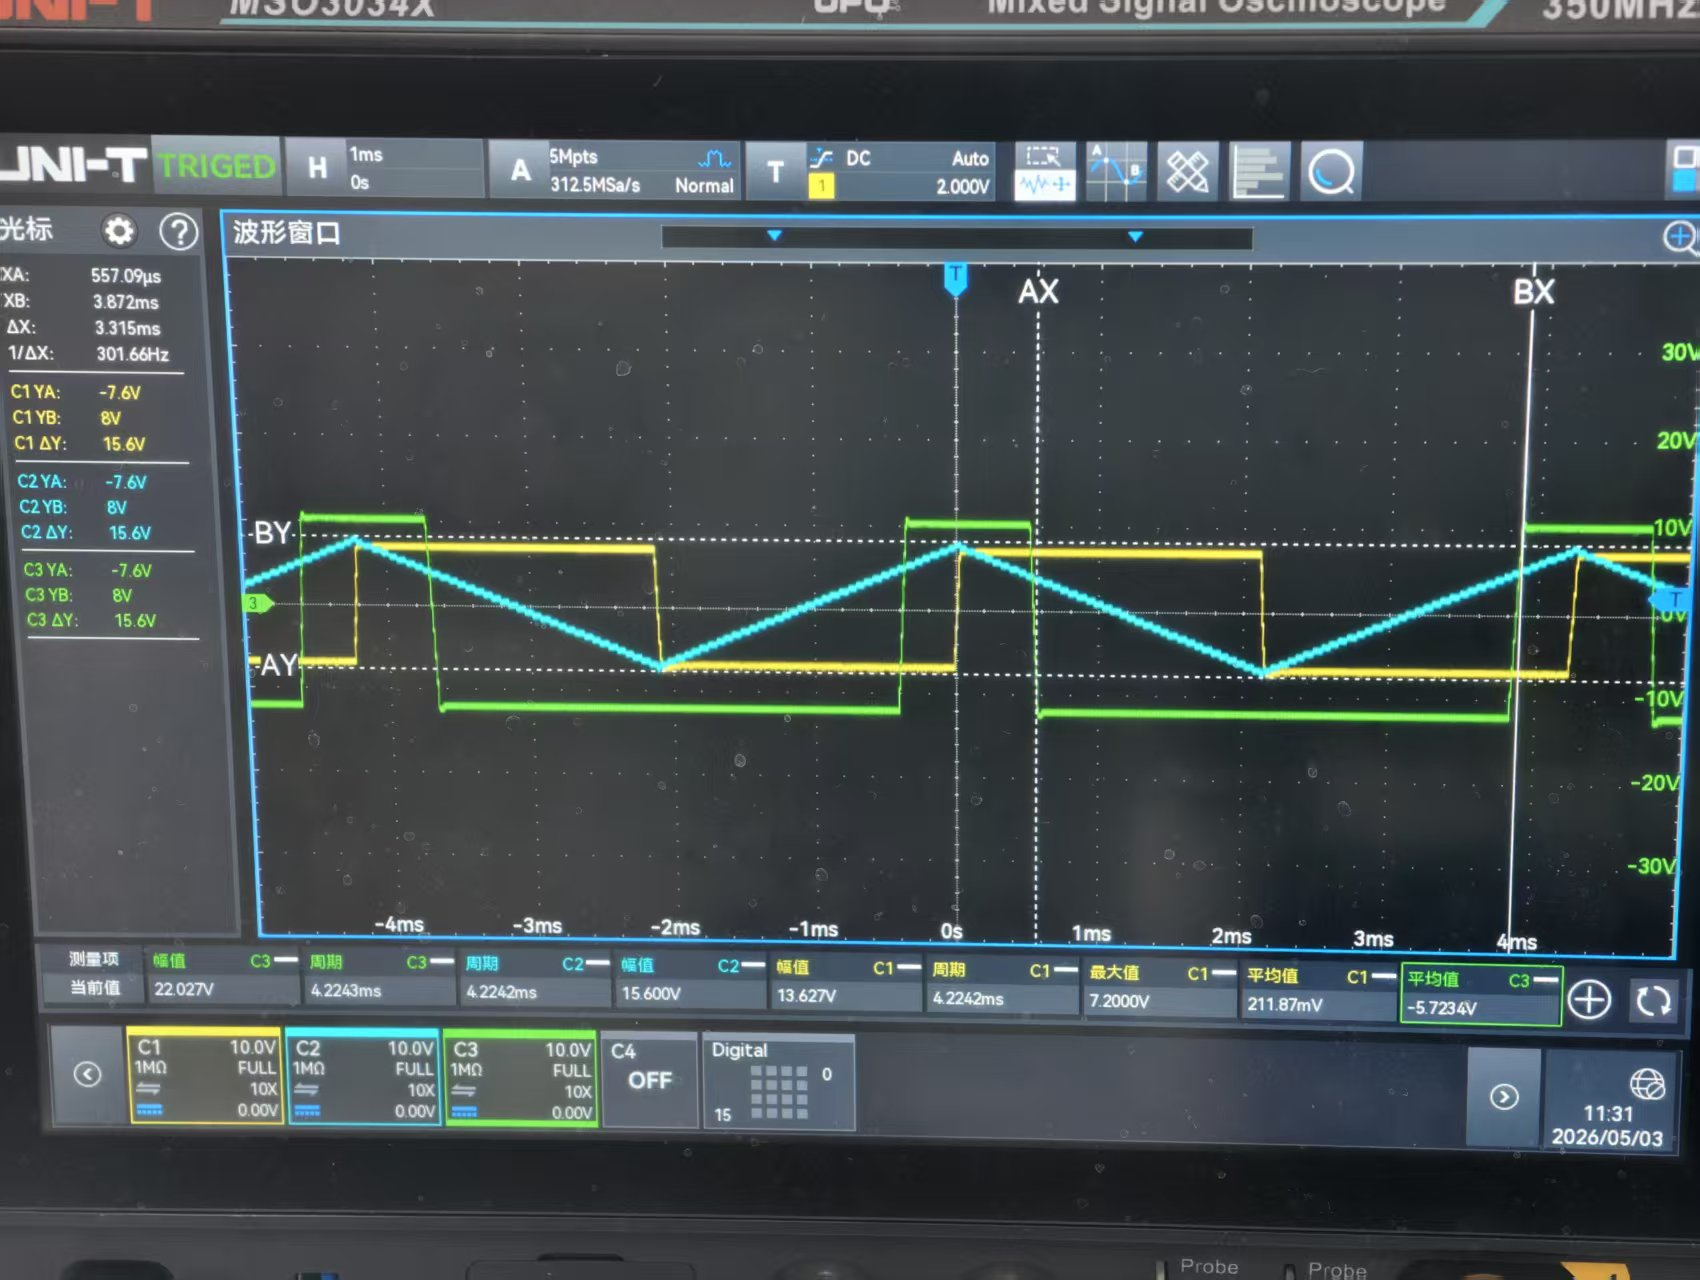
\includegraphics[width=0.45\textwidth]{figures/-4.jpg} 
    \caption{-4V时波形}
\end{figure}

\begin{figure}[H] 
    \centering 
    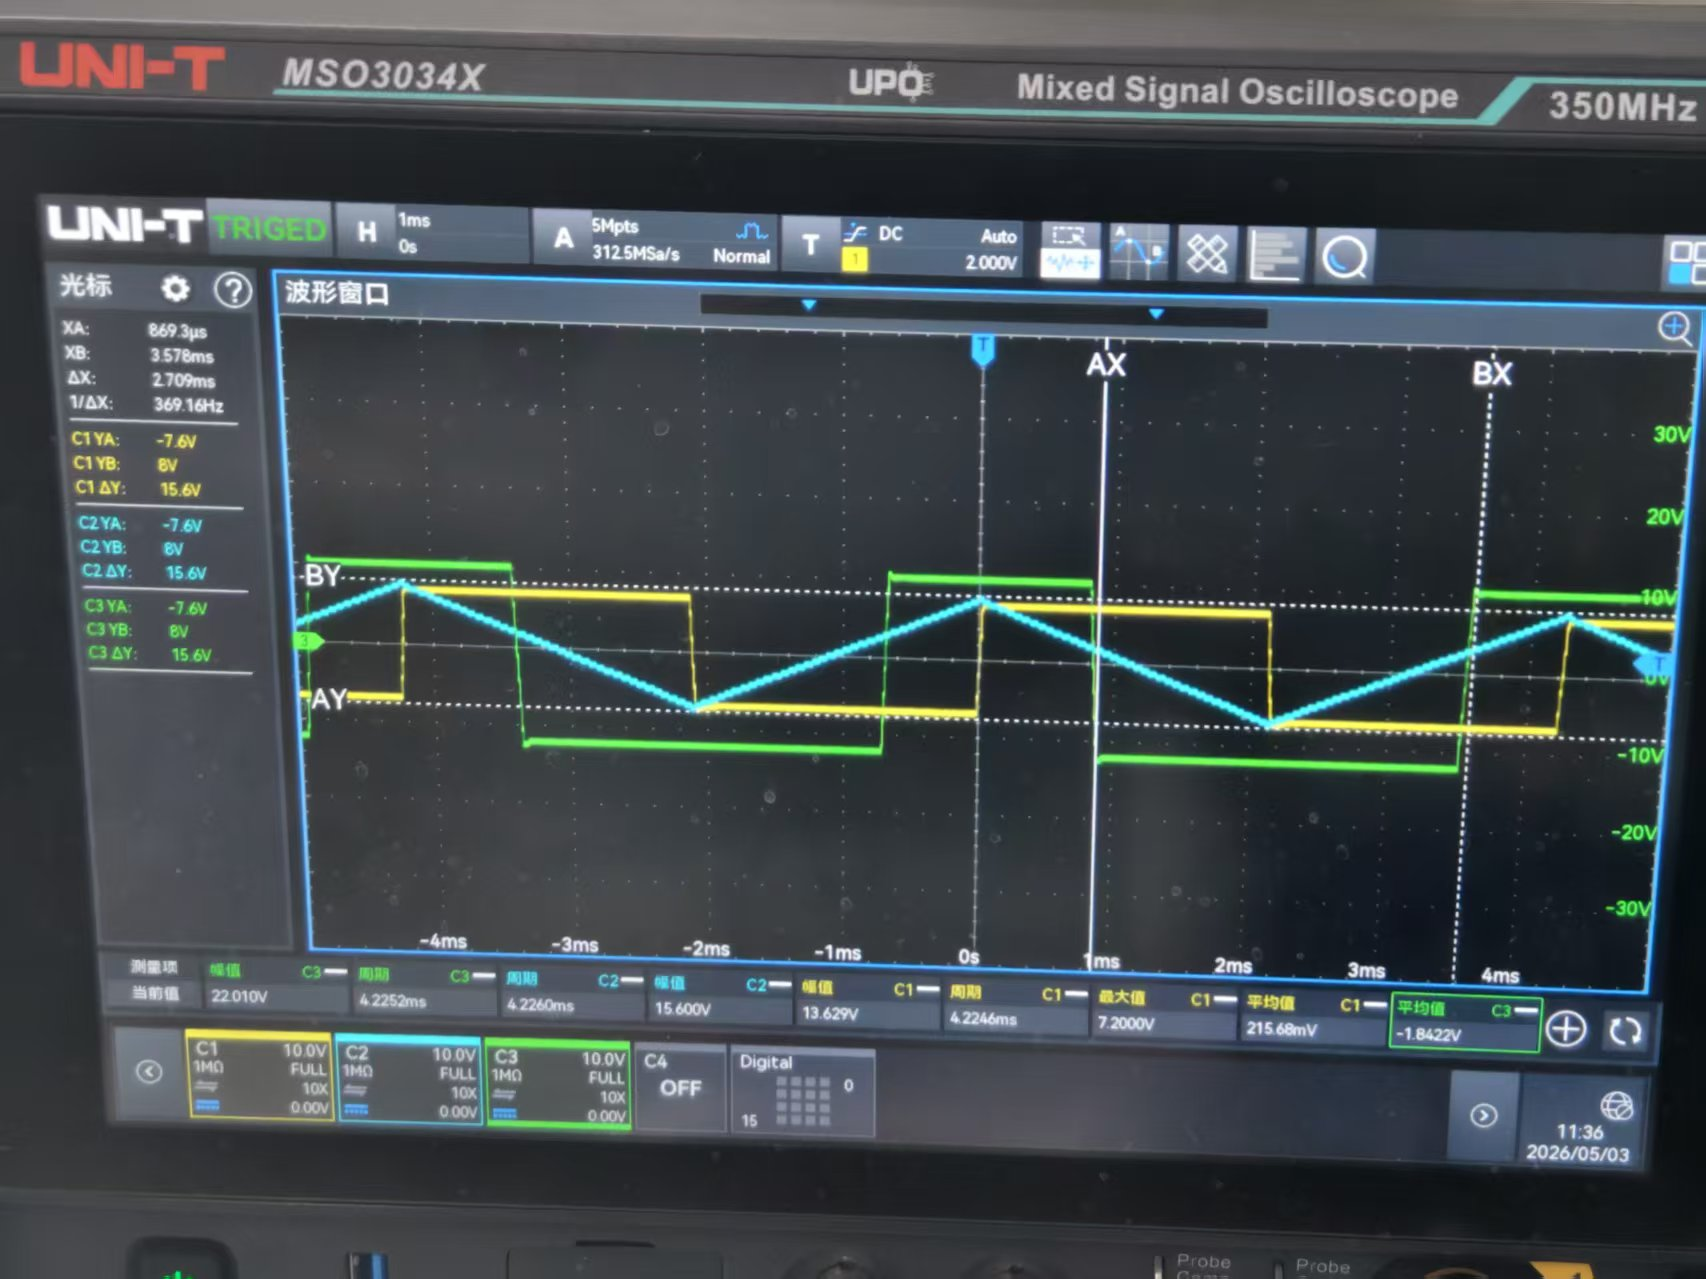
\includegraphics[width=0.45\textwidth]{figures/-2.jpg} 
    \caption{-2V时波形}
\end{figure}

\begin{figure}[H] 
    \centering 
    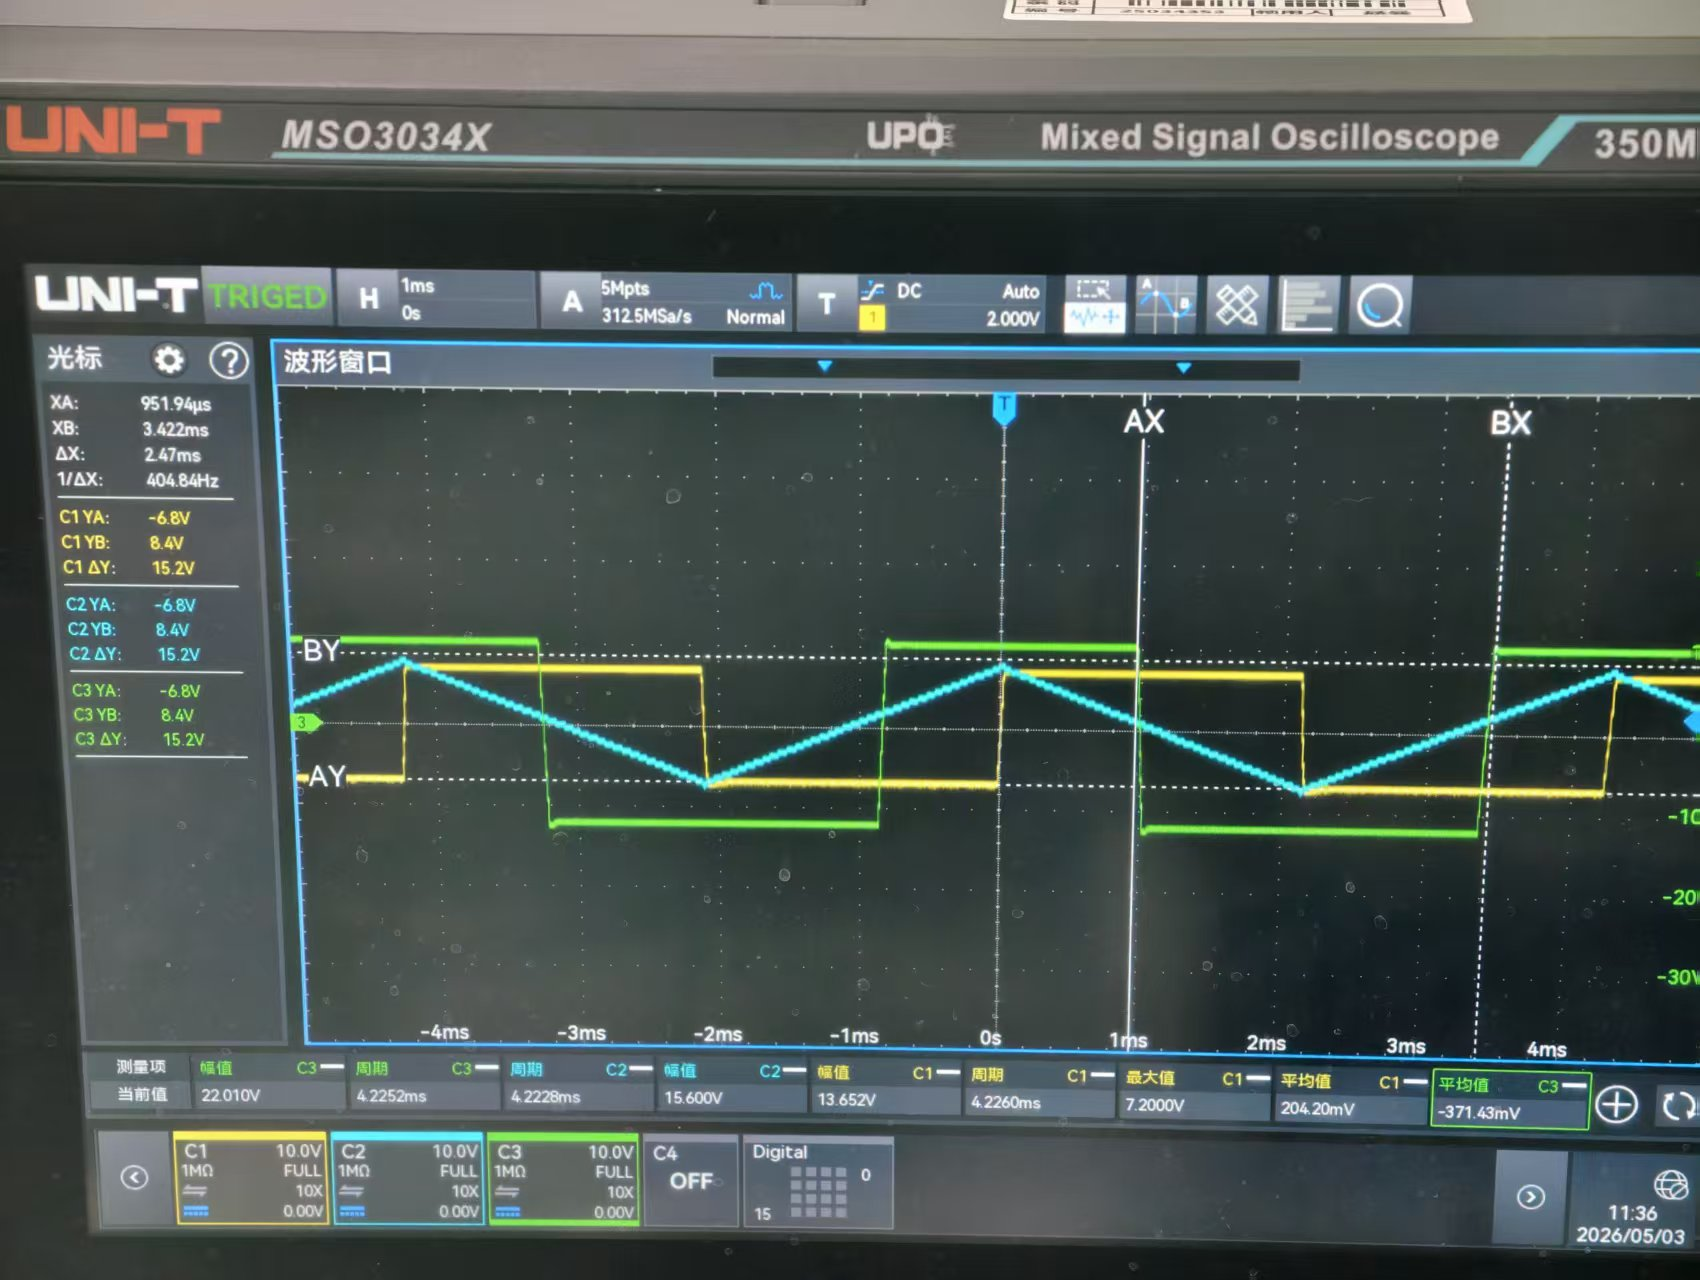
\includegraphics[width=0.45\textwidth]{figures/-1.jpg} 
    \caption{-1V时波形}
\end{figure}

\begin{figure}[H] 
    \centering 
    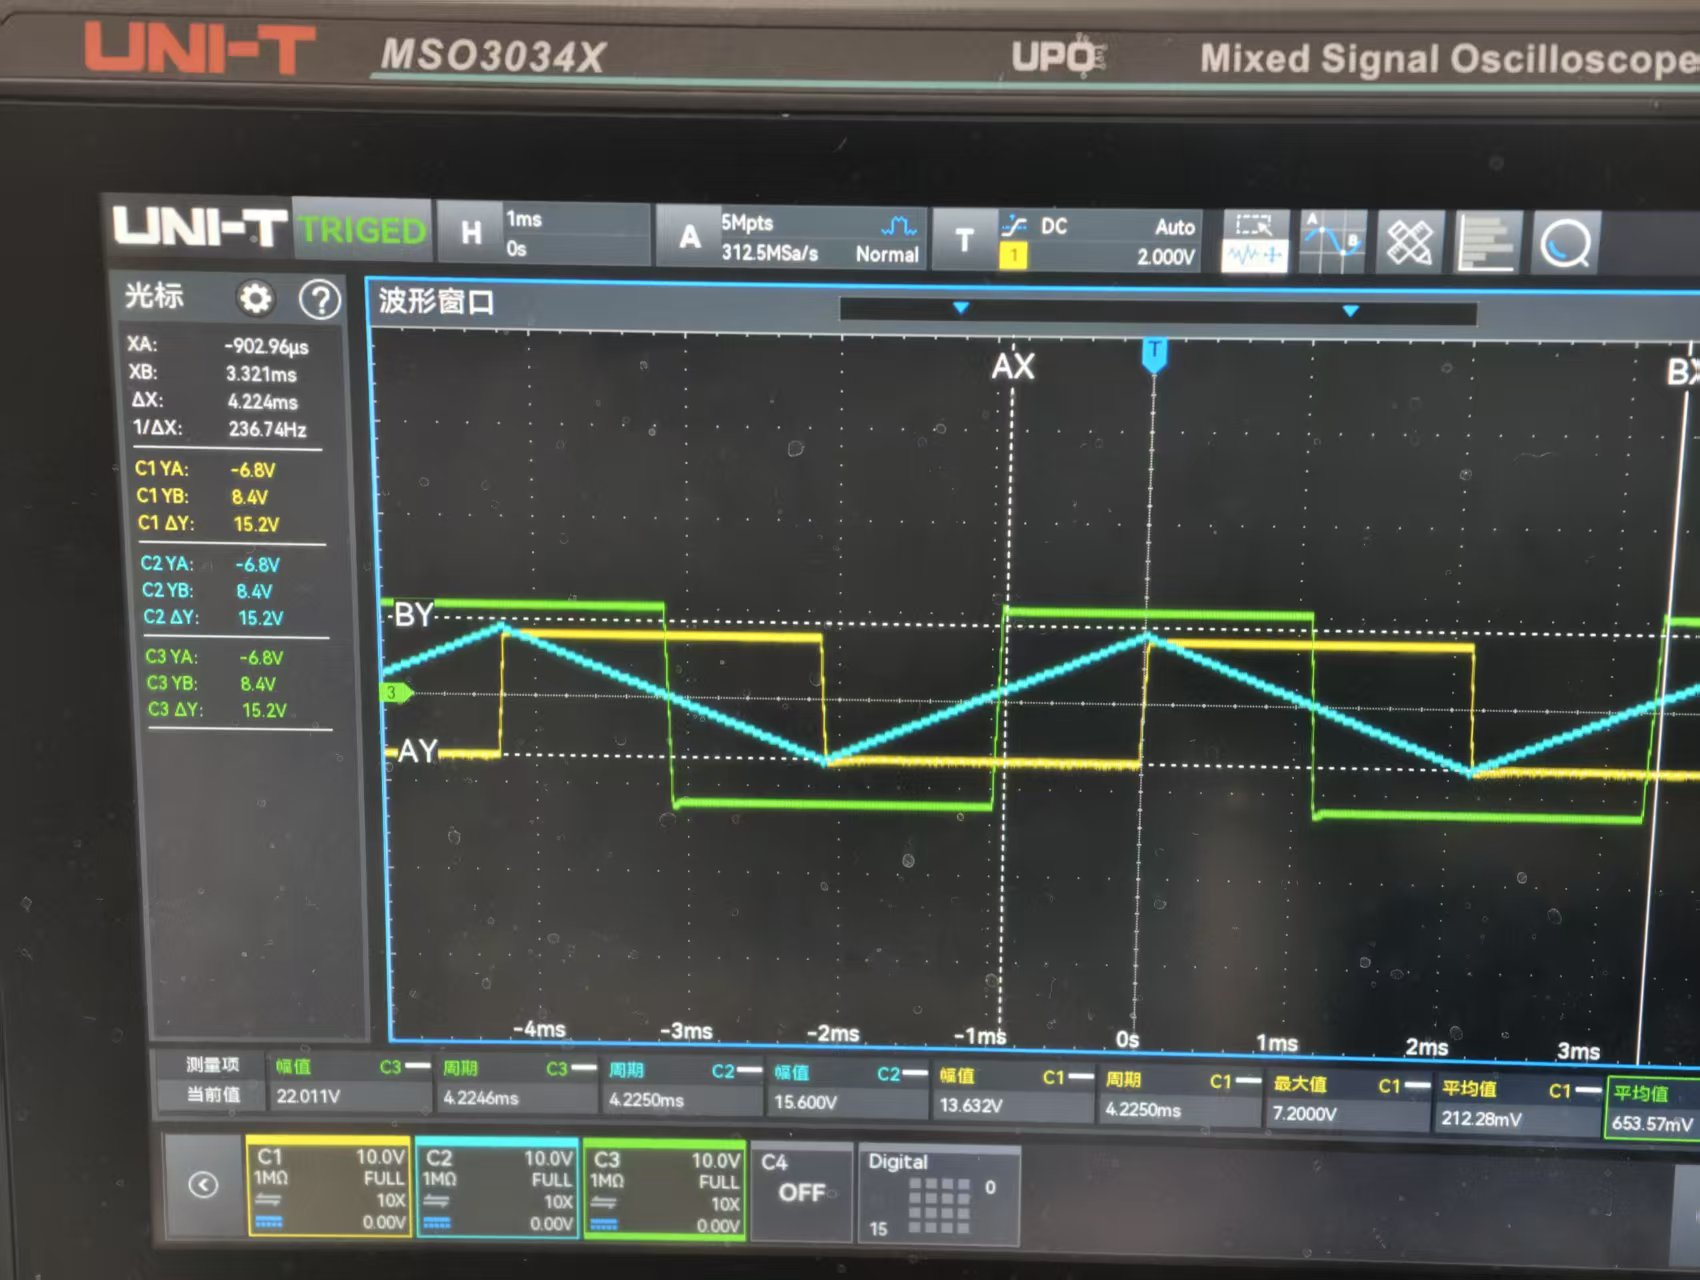
\includegraphics[width=0.45\textwidth]{figures/0.jpg} 
    \caption{0V时波形}
\end{figure}

\begin{figure}[H] 
    \centering 
    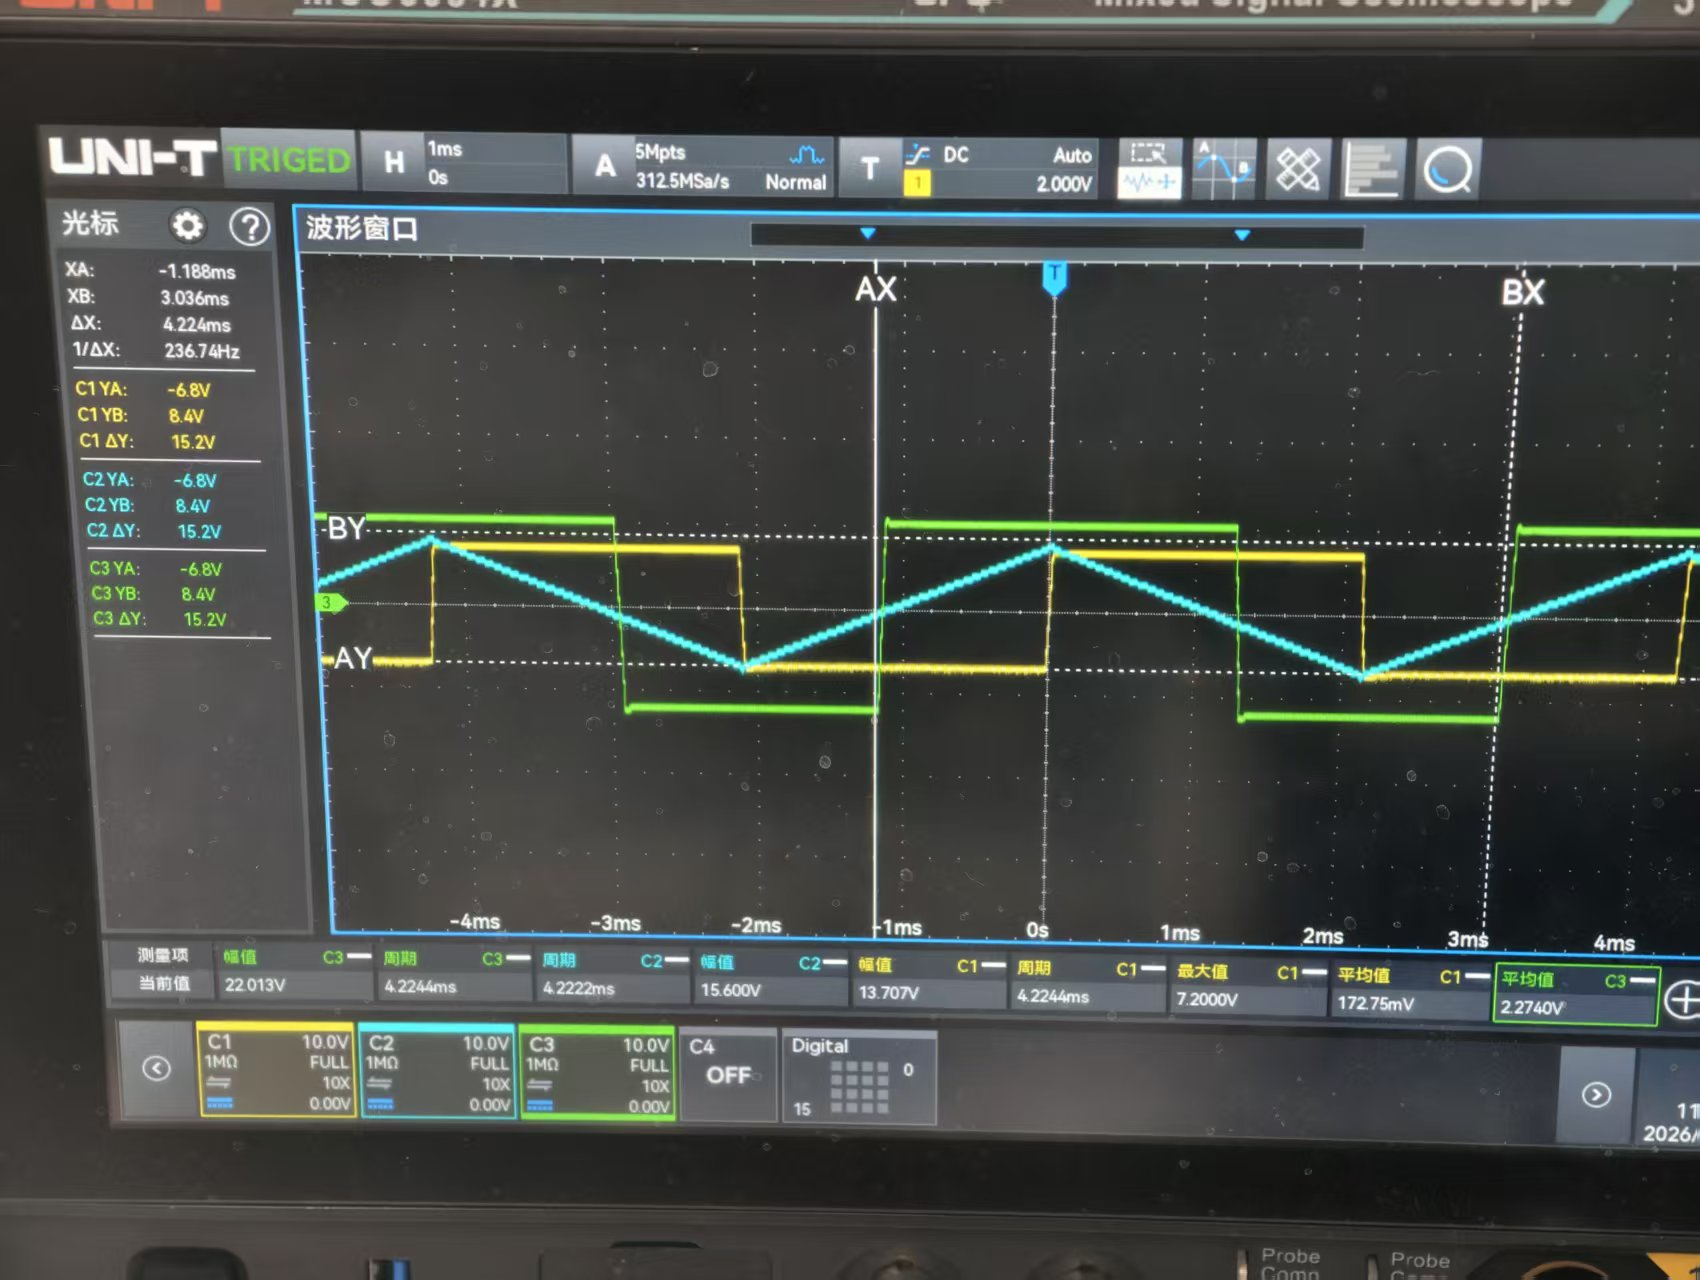
\includegraphics[width=0.45\textwidth]{figures/1.jpg} 
    \caption{1V时波形}
\end{figure}

\begin{figure}[H] 
    \centering 
    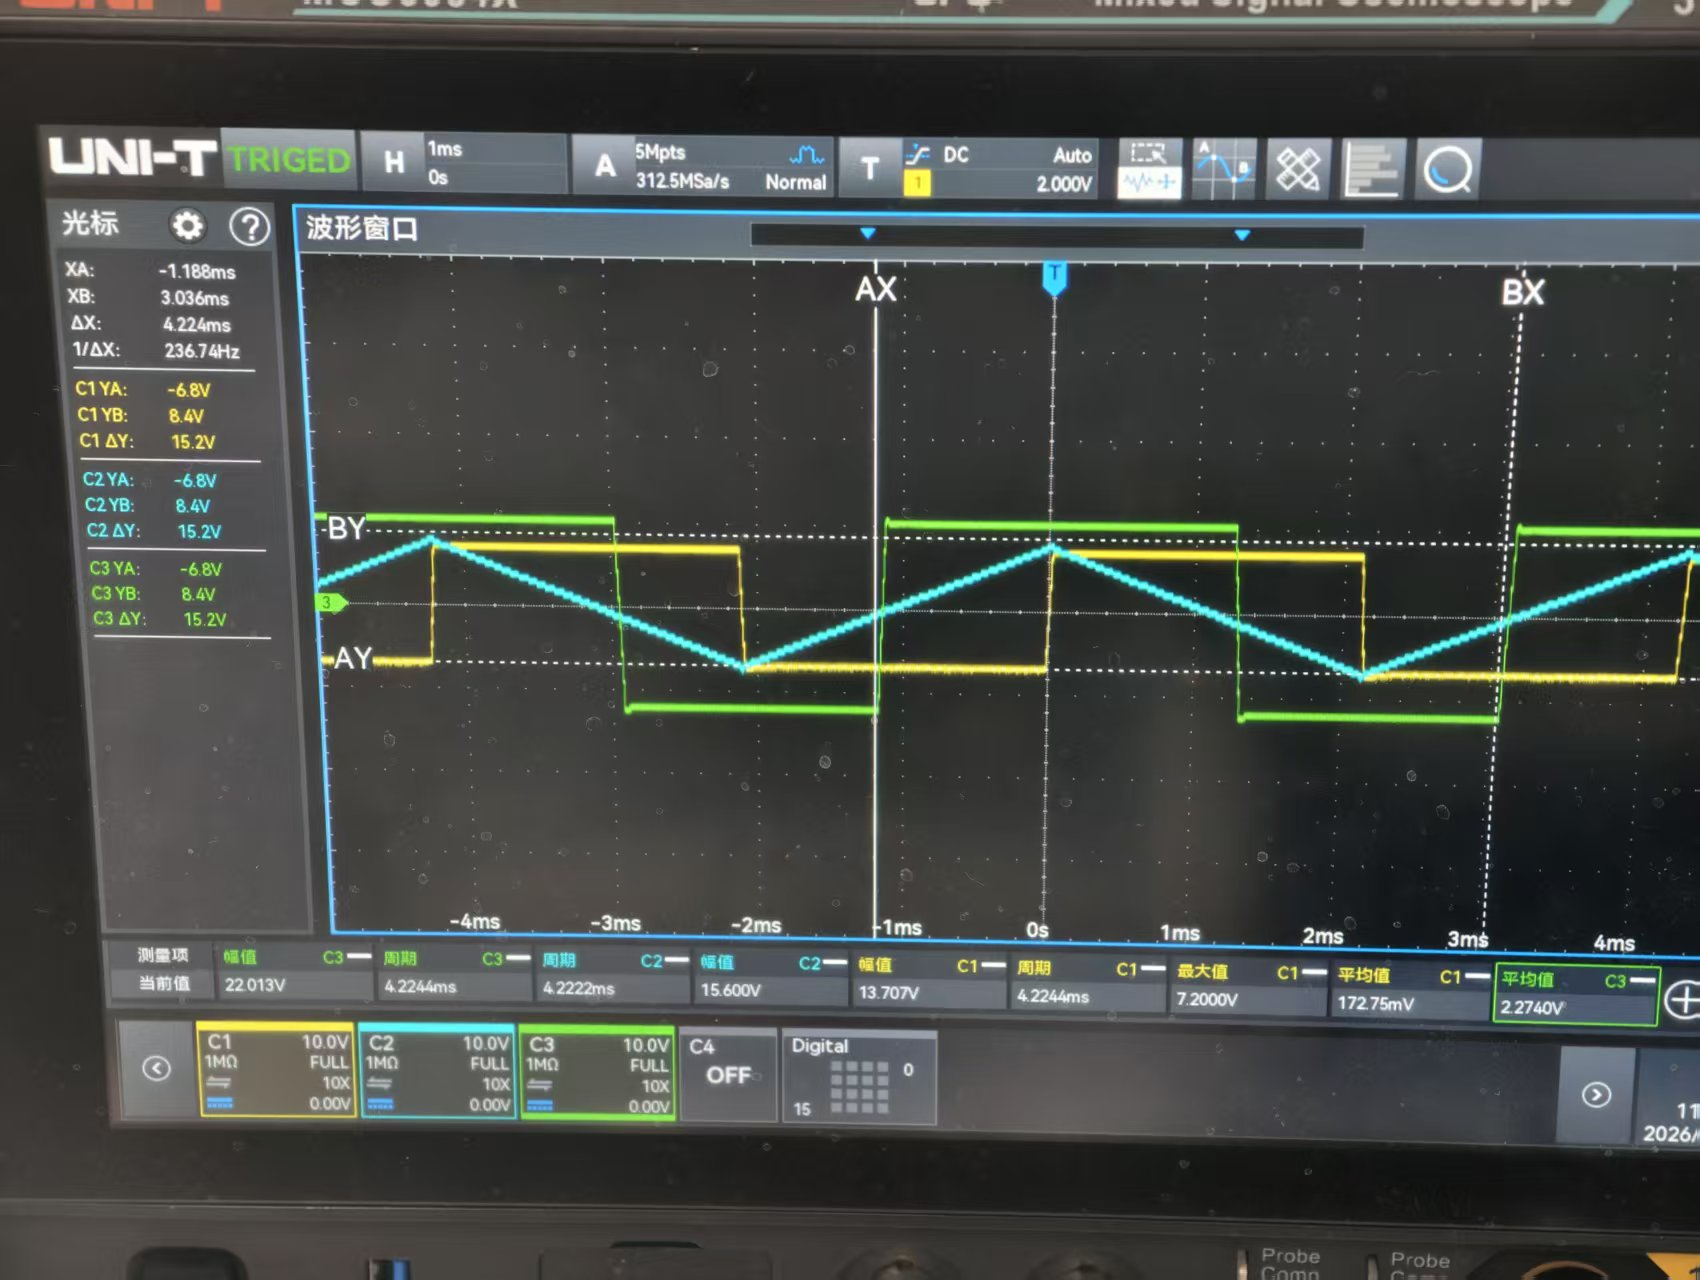
\includegraphics[width=0.45\textwidth]{figures/2.jpg} 
    \caption{2V时波形}
\end{figure}

\begin{figure}[H] 
    \centering 
    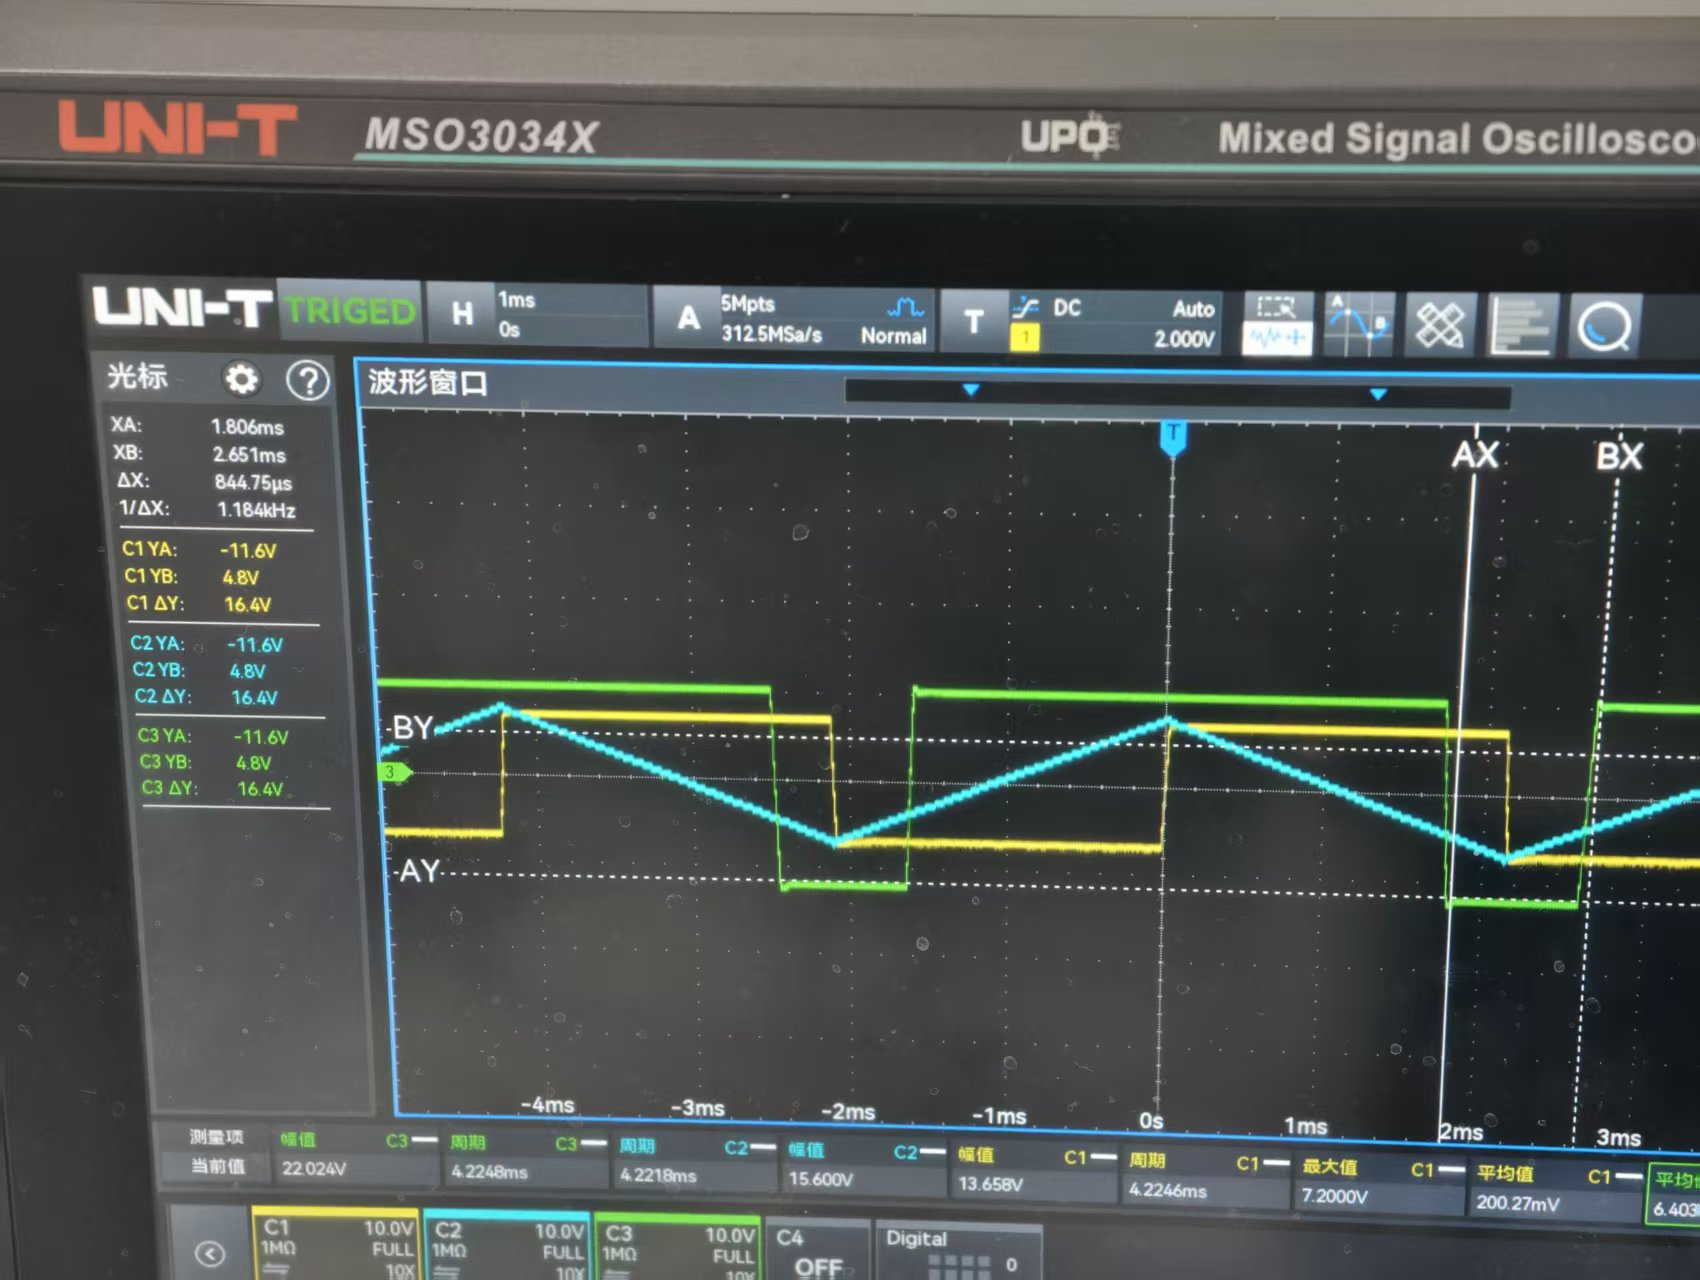
\includegraphics[width=0.45\textwidth]{figures/4.jpg} 
    \caption{4V时波形}
\end{figure}


\section{实验结果与分析}

\subsection*{1. 电路特点总结与数据分析}
根据实验1（1）的静态电压测试数据，当参考电压 $U_R=1\text{V}$ 时，输入电压 $u_i=0.5\text{V}$（低于门限）对应的输出为负饱和电压 $-10.7428\text{V}$，而 $u_i=1.5\text{V}$（高于门限）对应的输出为正饱和电压 $+12.1132\text{V}$，验证了电压比较器的开关特性：输入略高于门限时输出立即翻转为正饱和，略低于门限时翻转为负饱和。

在实验3的压控脉宽调制电路测试中，通过改变参考电压 $U_R$，实测占空比从 $U_R=2\text{V}$ 时的 $35.9\%$ 逐渐增大至 $U_R=-2\text{V}$ 时的 $64.1\%$（在低极值时可达 $80.0\%$），对应的平均电压 $U_{o3}$ 从 $-1.8433\text{V}$ 逐渐上升至 $+3.5556\text{V}$。这与理论规律一致：参考电压 $U_R$ 越小（向负方向移动），三角波高于参考电压的时间比例越长，输出矩形波的高电平时间变长，占空比和平均值均单调递增。

\subsection*{2. 波形与传输特性曲线讨论}
在实验1（2）的双踪观测中，正弦波信号通过比较器后被成功变换为了标准的矩形波。从实验1（3）在 XY 模式下观察到的电压传输特性曲线来看，其实测转折门限电压约为 $1.2\text{V}$，与理论计算的 $1\text{V}$ 存在微小偏差，这主要是由集成运放内部的输入失调电压引起的。此外，曲线的高电平（$+10.8\text{V}$）与低电平（$-12\text{V}$）绝对值不对称，这是因为实际运放的正负饱和压降本身就不完全对称。

\subsection*{3. 实测值与理论估算值比较}
以方波、三角波发生电路在 $R_{P1}=0$ 时的状态为例，已知此时电路的参数为：$R_1=100\text{k}\Omega, R_2=100\text{k}\Omega, R_f = R_5 = 100\text{k}\Omega, C_f = 0.01\mu\text{F}$。
根据理论公式，其振荡周期的估算值为：
\begin{equation*}
    T = 4R_f C_f \frac{R_1}{R_2} = 4 \times 10^5\Omega \times 10^{-8}\text{F} \times 1 = 4.0\text{ms}
\end{equation*}
示波器实测得到的方波与三角波周期为 $4.6320\text{ms}$，相对误差约为 $15.8\%$。该误差主要来源于实验箱上元器件（尤其是积分电容 $C_f$）的制造标称容差以及导线接触电阻。

另外，在实验2（3）调节 $R_{P1}$ 时，数据记录显示“当 $R_{P1}$ 逐渐调大，周期不断减小”。从理论公式 $T \propto (R_{P1}+R_5)$ 来看，阻值增大会导致充放电变慢、周期变长。实测数据与理论方向相反，查了一下发现很可能是实验箱的电位器旋钮方向标反了（旋钮刻度调大时阻值实际在减小），充放电反而加快，导致周期缩短。


\section{实验总结}

\subsection*{第一部分：思考题解析 (P172 四、2. 3. 4.)}
\begin{enumerate}[label=\arabic*., leftmargin=2em]
    \setcounter{enumi}{1}
    \item \textbf{图5.17-1(a)电路中若 $U_R$ 接地，分析输入为正弦波时输出为何种波形：} \\
    当 $U_R$ 接地时，电路即构成为过零比较器，门限电压为 $0\mathrm{V}$。当正弦波输入大于零时，运放输出正饱和电压（高电平）；当正弦波输入小于零时，运放输出负饱和电压（低电平）。因此，输出波形为\textbf{方波（或矩形波）}。
    
    \item \textbf{估算输出三角波和方波的频率，及改变波形频率和幅值的方法：} \\
    根据公式 $f = \frac{R_2}{R_1} \frac{1}{4 R_f C_f}$ 可以估算理论频率。
    \begin{itemize}
        \item \textbf{改变频率：} 通常可以通过改变积分电容 $C_f$ 作频率的粗调，调节可变电阻 $R_f$ 作频率的细调。此外，改变电阻比值 $R_2/R_1$ 也会影响振荡频率。
        \item \textbf{改变幅值：} 输出三角波的幅值主要由比较器的门限决定，即 $\pm \frac{R_1}{R_2}U_Z$（$U_Z$ 为稳压管的稳压值）。因此，改变电阻比值 $R_1/R_2$ 即可有效调节输出波形的幅值。
    \end{itemize}

    \item \textbf{预习思考题（4）解析：}
    \begin{itemize}
        \item [(1)] \textbf{图5.17-2电路中，$D_3$和$D_4$起什么作用？去掉会影响正常工作吗？} \\
        $D_3$ 和 $D_4$ 串接在供电回路中，起\textbf{电源防反接保护}作用。若不小心将电源正负极接反，二极管反向截止，可防止烧毁运放芯片。去掉它们后，只要电源极性连接正确，\textbf{不会影响}电路的正常工作。
        \item [(2)] \textbf{若 $D_1$ 和 $D_2$ 有一个击穿短路，输出 $u_{o1}$、$u_{o2}$ 变成怎样的波形？} \\
        若其中一个击穿短路，则该方向的稳压限幅作用失效，输出电压将被钳位在另一只二极管的正向导通压降（约 $0.7\mathrm{V}$）处。此时，$u_{o1}$ 将变成正、负半周幅值极不对称的矩形波；积分电路对其积分后，充放电速率产生巨大差异，$u_{o2}$ 将变成上升沿和下降沿斜率严重不对称的\textbf{锯齿波}。
        \item [(3)] \textbf{若将 $U_R$ 接地，$u_{o3}$ 输出矩形波的占空比为多少？} \\
        当 $U_R$ 接地时，比较器的参考电压为 $0\mathrm{V}$。因为输入的三角波信号 $u_{o2}$ 是以 $0\mathrm{V}$ 为中心上下对称的，占空比为 \textbf{50\%}（即标准方波）。
    \end{itemize}
\end{enumerate}

\subsection*{第二部分：实验体会与问题解决}

这次实验电路级数比较多，而且有闭环反馈，一开始我把三级全部接好再上电，结果示波器上什么波形都没有，查了半天也找不到问题在哪。后来拆掉 $A_3$，先只测前两级，很快就正常起振了，再接上 $A_3$ 也没有问题。以后遇到类似多级电路，还是应该一级一级分别调试。

另一个印象比较深的是实验2（3）。调 $R_{P1}$ 的时候发现电位器往大了拧，周期反而变小了，和公式 $T \propto (R_{P1}+R_5)$ 是反的。一开始以为是电路接错了，后来和同学讨论了一下觉得可能是实验箱上电位器的旋向标反了，实际拧大对应的是阻值减小。写报告的时候查了一下，确实很多老实验箱的电位器都有这个问题。


\end{document}

